% Use only LaTeX2e, calling the article.cls class and 12-point type.

\documentclass[12pt]{article}

% Users of the {thebibliography} environment or BibTeX should use the
% scicite.sty package, downloadable from *Science* at
% www.sciencemag.org/about/authors/prep/TeX_help/ .
% This package should properly format in-text
% reference calls and reference-list numbers.

\usepackage{scicite}

% Use times if you have the font installed; otherwise, comment out the
% following line.

\usepackage{times}

% The preamble here sets up a lot of new/revised commands and
% environments.  It's annoying, but please do *not* try to strip these
% out into a separate .sty file (which could lead to the loss of some
% information when we convert the file to other formats).  Instead, keep
% them in the preamble of your main LaTeX source file.

\usepackage{graphicx}

% The following parameters seem to provide a reasonable page setup.

\topmargin 0.0cm
\oddsidemargin 0.2cm
\textwidth 16cm 
\textheight 21cm
\footskip 1.0cm


%The next command sets up an environment for the abstract to your paper.

\usepackage{amsmath}
\usepackage{amsmath,amssymb}
\usepackage[section]{placeins}

\newenvironment{sciabstract}{%
\begin{quote} \bf}
{\end{quote}}


% If your reference list includes text notes as well as references,
% include the following line; otherwise, comment it out.

\renewcommand\refname{References and Notes}

% The following lines set up an environment for the last note in the
% reference list, which commonly includes acknowledgments of funding,
% help, etc.  It's intended for users of BibTeX or the {thebibliography}
% environment.  Users who are hand-coding their references at the end
% using a list environment such as {enumerate} can simply add another
% item at the end, and it will be numbered automatically.

\newcounter{lastnote}
\newenvironment{scilastnote}{%
\setcounter{lastnote}{\value{enumiv}}%
\addtocounter{lastnote}{+1}%
\begin{list}%
{\arabic{lastnote}.}
{\setlength{\leftmargin}{.22in}}
{\setlength{\labelsep}{.5em}}}
{\end{list}}

% Keywords command
\providecommand{\keywords}[1]
{
  \small	
  \textbf{\textit{Keywords---}} #1
}


% Include your paper's title here

\title{Interim Report} 


% Place the author information here.  Please hand-code the contact
% information and notecalls; do *not* use \footnote commands.  Let the
% author contact information appear immediately below the author names
% as shown.  We would also prefer that you don't change the type-size
% settings shown here.

\author
{Radek Chramosil\\
\\
\normalsize{WorldQuant University}\\
\\
\normalsize{E-mail:  radek@keemail.me}
}

% Include the date command, but leave its argument blank.

\date{}



%%%%%%%%%%%%%%%%% END OF PREAMBLE %%%%%%%%%%%%%%%%



\begin{document} 

% Double-space the manuscript.

\baselineskip24pt

% Make the title.

\maketitle 



% Place your abstract within the special {sciabstract} environment.

\begin{sciabstract}
This document is the Interim Report for the Capstone Project. It shows the basic structure for the database that holds data the data from crypto-currency exchange Binance and some initial data analysis.
\end{sciabstract}

\keywords{High frequency trading, Market microstructure, Algorithmic trading}


% In setting up this template for *Science* papers, we've used both
% the \section* command and the \paragraph* command for topical
% divisions.  Which you use will of course depend on the type of paper
% you're writing.  Review Articles tend to have displayed headings, for
% which \section* is more appropriate; Research Articles, when they have
% formal topical divisions at all, tend to signal them with bold text
% that runs into the paragraph, for which \paragraph* is the right
% choice.  Either way, use the asterisk (*) modifier, as shown, to
% suppress numbering.

\section*{Introduction}
The structure of the database is described below. Additionally,  I provide more details about the data analyses so far carried out as well as some suggestion for trading possible trading strategies. Some plots for second data set are provided. The asset I worked with is \textbf{TUSDBTC} as quoted on \textit{Binance Exchange}. The asset is Bitcoin quoted in USD. The access to the full exchange is free and level 2 data is available for every tick. The data was collected on second basis for one hour. The collection was done with 1 second frequency as opposed to per trade basis (I am still unsure how to handle data collection per trade basis). The data set is therefore some 3440 full market book hits; some 100 quotes for bid prices and some 100 quotes for ask prices.

\section*{Research Topics}
This sections highlights some issues in the so called capital market micro-structure. I focus on technical aspects mostly. It is often difficult to identify or read about the specifics, say, of an API as used by some exchange. So, I use my work on Bitcoin and Binance exchange as an example. I mostly focus on discuss about US stock market as this is the most commonly discussed topic in the literature. This is continuous action order-driven market.  I provide the time units definitions for convenience.

\begin{center}
\begin{tabular}{|c|r|} 
\hline
\multicolumn{2}{|c|}{Second to lower time intervals} \\
\hline
1 second & 1 000 milliseconds \\ 
1 second & 1 000 000 microseconds \\ 
1 second & 1 000 000 000  nanoseconds \\ 
\hline
\end{tabular}
\end{center}


\subsection*{Electronic Trading Chain}
There are many aspects that can be discussed with regards to trading chain links between brokers, exchanges, investors (retail, institutional or algorithmic trading engines). However, Durbin \cite{durbin} mentions that for for a high frequency firm access the exchange for two reasons only. One is to submit their trade flow (trade execution) and the other is the receipt of market data. This can be generalised to any market participant. Hence, I provide the Figure \ref{fig:market} that shows high level overview.

\begin{figure}[h!]
	\centering
  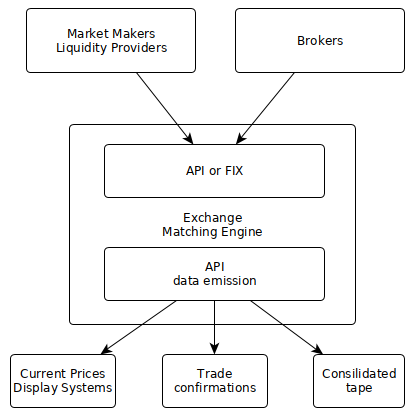
\includegraphics[scale=0.6]{market.png}
  \caption{Market Structure Overview}
  \label{fig:market}
\end{figure}

\paragraph*{Matching Engine} The core about any trade linking the matching mechanism. Johnson \cite{johnson} provides high level structure for the matching engine. Each order (that is price and quantity for bid or ask) is processed as it arrives to the matching engine. The below steps are taken each time there is a new order.
\begin{itemize}
\item The order instruction is added to internal order book
\item Trade matching rules are then used to see if any matches are now possible
\item The order book is updated to reflect any changes
\item Execution notifications are sent to any result matches
\end{itemize}
These steps essentially are the core of any order driven market. Figure \ref{fig:lse} shows how LSE displays their market order book to their clients \cite{lse}.

\begin{figure}[h!]
	\centering
  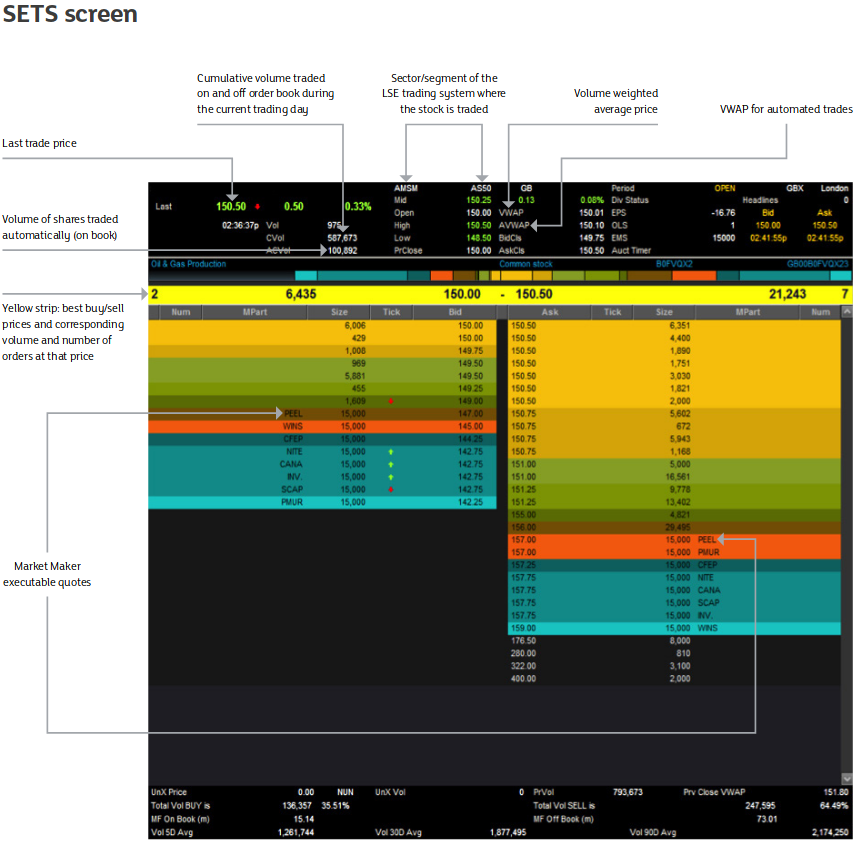
\includegraphics[scale=0.55]{lse.png}
  \caption{LSE Market Order Book screen}
  \label{fig:lse}
\end{figure}


In an attempt to assess how this matching algorithm might work, I used Binance exchange as an example. This exchange sees the order book at a new state each time there is an order and uses a data field 'UpdatedID' to mark this state. The exchange members are the able to request the order-book state stamped by this ID. Binance uses only REST API which we can query programmatically, say using Python's Requests package. On the contrary, on the NYSE's website we can read about different services this exchange offers to their clients \cite{nyse}. We see that they have an event-based depth of book feed available, which is not something Binance offers as yet. Programmatically, event driven API would be a better option for us, however we can expect that NYSE charges their fee for this service.

To understand how to classify the different levels of service an exchange might provide, it is useful to consider the latency differences. O'Hara \cite{ohara} provides a good summary of services for Tokyo exchange. This exchange offers Arrownet, the standard service, which has the latency of several milliseconds. Their priority service allows users to place devices at data center entry points for their network, lowering the latency to  260 microseconds. Finally, the co-location at their primary side offers 15.7 nanoseconds service. We can learn from this that the simplest and most straight forwards way to classify the services the exchange provide is based around the time latency. Unfortunately, the exchanges are not transparent around the latencies. NYSE does not talk about latencies at all on their website \cite{nyse}. Binance simply leaves this issue to the market participants as any one can access their matching engine over the Internet.

Further, the important aspect of co-location is that once co-located the market participants have the cable of the same length, see the interview with Manoj Narang \cite{reuters}. Once, we pay for the co-location service, we should have the same delay as anybody else who pays for the service.

Financial Information Exchange protocol (FIX protocol, see Johnson \cite{johnson} for details, it is just a version of XML) and exchange application programming interface (API) provide a way to submit orders. The broker orders as as well as market makers therefore must reach the matching engine the same way even though that the difference is that some people press buttons on their screen and some people monitor the market programmatically and their programme will submit the order. It only that seems to matter is the latency. FIX should be slower as it needs to interpreted as opposed to and API but it is used as it is common to the whole market. Johnson also \cite{johnson} mentions exchanges have separate servers for processing orders and emitting data. We would have to investigate what a specific exchanges does before we start trading.

After a trade is submitted to the machining engine, the machining engine must make its state available to the market, specifically market maker, broker, data vendors or authorities. This includes trade confirmation but also open orders as well as the matched trades. In the US an exchange may submit the confirmation firstly to Consolidated Tape Authority (CTA) - see Durbin \cite{durbin}. CTA then in turns should have all market data and some hedge funds use it as a data source. While Europe is missing the consolidated type all together as suggested by O'Hara \cite{ohara}. Perhaps, the rest of the world faces this issues too.

\paragraph*{Brokers} The traditional way for people to access the market is over the phone via a broker; refer to Harris \cite{harris} to see what specific applications or systems are involved. I just mention that in the principle for the order-driven market the order must end up in the same order book. However, brokers actually root the market order to the venue that pays them the most, see Harris \cite{harris} or O'Hara \cite{ohara}. O'Hara mentions that there are some 15 different stock exchanges and 50 alternative venues.
In order for the broker to give their clients competitive edge over poor algorithmic trades, brokers now offer algorithmic execution for trades as well. As en example, I look into Investment Technology Group's (ITG) executions strategies \cite{itg}. Their clients can benefit from a large variety of  different execution algorithms or build their own. ITG also DMA in some forms. So, we see that the playing field is levelling up even for retail traders.

\paragraph{Algorithmic Trading Engines} The structure for an algorithmic trading engine is reasonably well described by Durbin \cite{durbin}. He provides summarises his ideas in the below flow chart in Figure \ref{fig:component}.

\begin{figure}[h!]
	\centering
    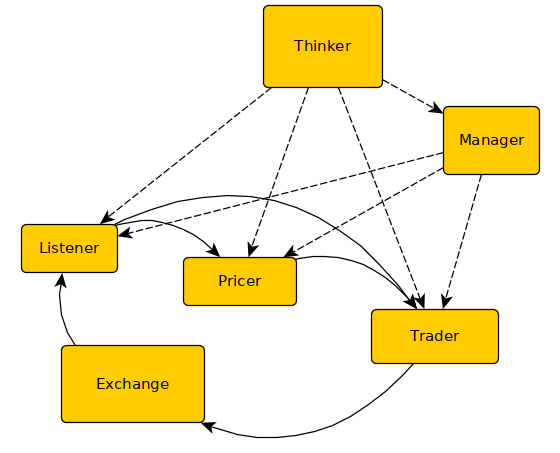
\includegraphics[scale=0.55]{component.png}
    \caption{High Frequency Trader - Operational Structure}
    \label{fig:component}
\end{figure}

He defines the terms in the following. \textit{Thinker} take direction from humans. This would GUI for the application. \textit{Manager} controls on the other components. So, this would be the main server or the main program that oversees all the programs. Then again we have \textit{exchange}. This is the matching engine as discussed above. \textit{Listener} takes in the market data and make them available to other components. Durbin states that this should sit as close as possible the market data source (exchange or CTA) and take in every tick. Listener also does checks for errors or arbitrage if multiple sources disagree. \textit{Pricer} Durbin states that this component calculates the price of assets in the real-time however we know that we could use any strategy or use any mathematical model here, not just pricing. This application or a function receives the inventory information from \textit{Manager}. \textit{Trader} submits/cancels the orders in the exchange. Finally, \textit{Manager} is a program that controls all the other components.

We can see how a general algorithmic trading operation may run from Durbin's discuss, however we know that the reality of algorithmic trading is more complicated than that. We also see that this structure fits well into our discussion well, see Figure \ref{fig:market}. Further, Johnson \cite{johnson} provides code C++ snippets that can be established in individual components.
\paragraph{DMA Services} Johnson \cite{johnson} provides a good definition for Direct Market Access (DMA), DMA means that a computerised system is reponsible for executing the orders to buy or sell a given asset, rather than being worked manually by a trader. It should be noted that the broker can give their client this access rather than the exchange itself, however many exchanges give DMA to their market makers. In all my discussion, I assumed DMA as the whole market shifts towards computerised systems anyway. 
\subsection*{Benefits and Pitfalls of DMA technologies}
\paragraph*{DMA Types} Johnson \cite{johnson} provides a good overview of DMA services available. I just provide a brief definitions and suggest a way how we should study the pros and coins as market participants.

\paragraph*{Direct Market Access} In section, we define \textit{Direct Market Access} (DMA) as the situation when broker's client makes use of the brokers infrastructure to send the orders to the exchange, like broker's own orders. \textit{Sponsored Access} term is used when the broker's client is given broker's access credentials to execute the trades directly at the exchange, but not having to use the broker's infrastructure. This should be faster however there is some connection overhead for the broker to monitor the trading to prevent any excessive risk taking by the client. \textit{Crossing} refers to the situation when brokers offers the access to the dark pool to their clients. This, Johnson claims, to be used when a client is looking to carry out a large trade and is trying to hide it from a many market participants that are able to respond to the orders visible in exchange order book. \textit{Direct Liquidity Access} is then the term when the broker offers the access to dark pools and to the exchanges at the same time. In addition, some brokers started to use the term \textit{Direct Strategy Access}. This means broker provides their client with execution algorithms.

Thus, we see that the way to compare different ways to access the markets can be classified by
\begin{itemize}
\item latency,
\item venue availability,
\item execution algorithm,
\item price.
\end{itemize}
We would need to research what specific deals are available to us from different brokers and decided on the best deals based on the above criteria.

One final thought about DMA comparison is that in case of crypto-currency market, there are no brokers at all. One additional form of DMA is not have a broker.

As for the benefits, the obvious case for them that automated markets are more efficient so cheaper, that is the trading is cheaper, which was the original cause for automation, see Patterson \cite{patterson}. This authors talks about the fact that NASDAQ market maker kept their spreads artificially high in the past. The solution was to automate the trading. Also, one more obvious benefits is that direct market access provides greater transparency with regards to the price data and well as market order book. The exchange members can request all the data their desire, however in case of standard capital markets this subscription is paid. DMA technologies may allows us to bypass brokers, who often have a lot conflicts of interest with respect to their clients (broker can sell their client order flow or they execute market orders on behalf of their clients when they deem that the position is too risky and collect the trade fee). This is the case in the crypto-currency space. In addition, we test trading strategies under live access to the market.

On the other hand, the market automation created problems at the same as it had provided us with benefits. Exchanges now sell access to a public information, they sell access to the market order book with difference latencies. As a results, they turn public information into private information for time intervals measured in microseconds or nanoseconds \cite{ohara}. In fact Brad Katsuyama claimed in his interview with BBC that the exchanges make more money by selling high speed data and technology than they make by matching trades . It is clear that some market participants benefit from this latency advantage at expense of the market participants that did not pay for the low latency access, see Patterson \cite{patterson}. Another problem is that the matching engines are not publicly available in standard markets, maybe not in some obscure crypto-currency open-source space. What this means that the exchange can create or special hidden order types, which are again given just to some specific market participants and the other may not know this, see Bodek \cite{bodek}. This author and active market participant claims that his algorithmic trading operation went in the red as he did not have access to the hidden marker order types while his competitors had. He talks about hidden Alphas in different order types. So, we that the problem is actually the fact that the matching engine is not public information just the API is.

Therefore, we can see that algorithmic trading creates transparency as more data is available now while at the same time it does exactly the opposite in some other sense.
\subsection*{Risks in DMA}
DMA does have obvious risks. Knight Capital lost \$440 million in trading loss due to a bug in their systems \cite{nytimes}. The company suffered power disruptions and it was not able execute orders on some other day. AXA Rosenberg lost \$217 million in client money due to an error in their model for managing risk \cite{cbs}. So, we see that one of the big problems and risks with DMA is the coding errors.

Further, the all technical risks that linked to running a data centres such as power shortages, car or track accidents causing evacuation of the area, flights patterns, flat plains, nuclear plants, rail lines, crime level and even light night strikes. All of these events could cause an outage in a data facility \cite{vpro}. DMA is directly dependent on all of these as it is carried out in the data centres physically next to where the matching engine server is located. In case of computer networks, we need to add risk that the connections may fail for the same reasons and many other as in case of a data centre.

As previously mentioned, we do not have a full access to the matching engine, so we run a risk that the exchange gives better order types so users over as another users.

There are also topics such as slippage, front-running, quote-staffing (see, Durbin \cite{durbin}), however there are more general to the market structure not to the DMA itself.
\subsection*{Latency Types}
The basic ideas behind the latency issue are well summarised by Kirilenko \cite{kirli1}. He points that a standard way to measure latency is by determining the time it takes a given message to travel from source to destination and back - \textit{round-trip time} (RTT). he talks about
\begin{itemize}
\item \textit{communication latency} - can be reduced by co-location
\item \textit{market feed latency} - can be reduced by buying proprietary data feed
\item \textit{trading platform latency} - cannot be reduced by a trader, taken as given
\end{itemize}
Kirilenko and Lamacie \cite{kirli2} also points that the latency is a random variable as in Figure \ref{fig:latency} where we can guess what the distribution properties are.

\begin{figure}[h!]
	\centering
    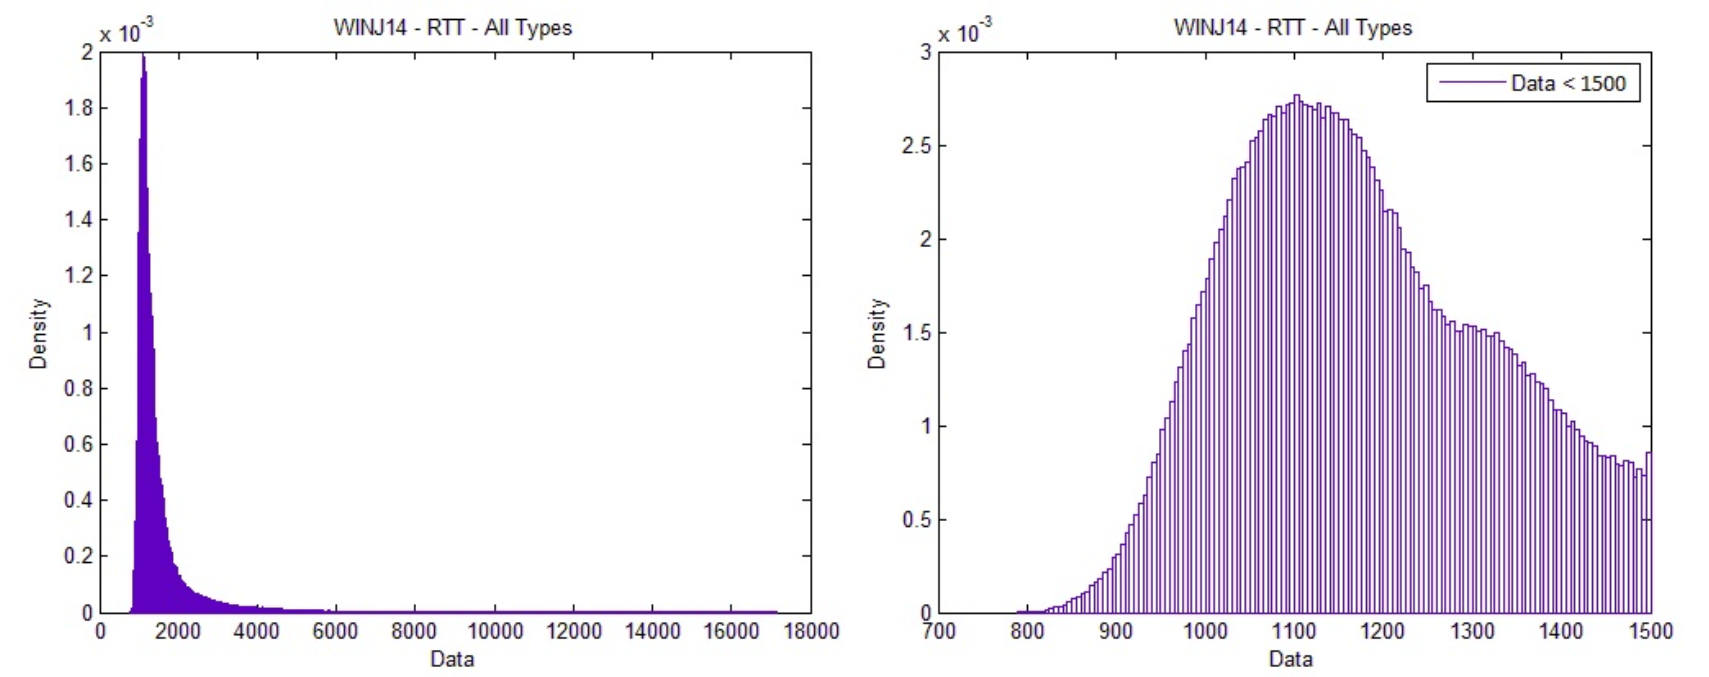
\includegraphics[scale=0.27]{latency.png}
    \caption{RTT - All Types: Submissions, Modify, Cancel - from \cite{kirli2}}
    \label{fig:latency}
\end{figure}

Further, we can break down the latencies in a different way. Kumar \cite{kumar} provides a useful overview of how trading system latencies can be defined and measured. He summaries the problem at hand as:
\begin{align}
\text{Trading System Latency} & = \text{(All the processing node latencies)} \nonumber \\
  & \qquad + \text{(Operating system network stack latencies)} \nonumber \\
  & \qquad + \text{(The entire network device latencies)} \nonumber \\
  & \qquad + \text{(The entire wire time latencies)} \nonumber \\
  \nonumber
\end{align}
Kumar \cite{kumar} then defines:
\begin{itemize}
\item \textit{Processing node latency} is the time spent within the application business rules and logic.
\item \textit{Operating system network stack latency} is the time spent within operating system calls and hardware network interfaces.
\item \textit{Network device latencies} is the time spent in networking equipment (load balancers, firewalls and routers).
\item \textit{Wire time} is the time it takes for a message to transmitted on a physical medium. Specifically, a foot of a cable equates to a nanosecond \cite{bbc}. It is 50 to 55 micro seconds to data to travel one way on 10 km of fiber optic \cite{kumar}.
\end{itemize}
This discussion shows that to reduce the latency within a computer system that we need to drill into every step our computer does along the way between the the computer and the matching engine. That we would have to use the most efficient algorithms and data structures to handle the processing node latency. The industry uses real-time operating systems \cite{durbin}. Alternative way to use the just a chip set without the operating system. Wire lengths are reduced by co-location. The work documented by Algo-Logic may serve as a good example \cite{lockwood}.

It is worth noting that a lot of low latency issues are linked to the US equity markets and the equity instruments that have multiple venues which then leads to the latency arbitrage, however one way to solve this is to just use instruments that have only one trading venue. We may stay from the race altogether. As a result, HFT firm may build its business around mathematical modelling, see how the company called RSJ does the business \cite{rsj}.
\subsection{Typical Order Messaging System}
I was not able to any specific information with regards to type order messaging process - Order Request, Data Conversion, Order Enrichment, Order Transmission and Exchange Acknowledgement for any standard exchange. The Investor Exchange provides REST API \cite{iex} for the data but not for orders. We check how to communicate to Binance exchange using a python package \cite{bapi}, however that is also REST API.

We are left with general suggestions about how to reduce latency. C++ is seen as the fastest language that gives control over the computer at very low level (memory pointers, memory management). Generally, it is good to keep the data in memory as well so many algorithmic trading operations use KDB, which is a in-memory relational time series database. The coding style should be modular and functional as opposed to object orientated as inheritance slows the program down. In addition, jobs like error handling comes with an overhead. So, more steps in the code, the better enough though we might be short on standard coding practices. As for operating system, Durbin \cite{durbin} mentioned Linux (CentOS is mentioned by Lockwood \cite{lockwood}). However, we still should remove a lot of  
functionality, such as a graphical interface, for the server where would trade from. The point is that we wish to run our application instantaneously and at the constant time. We wish to remove as much randomness from our latency as possible. So, we can control the system. Obvious options to consider are parallel processing within a single server. This is both CPU multi-threading (Durbin \cite{durbin} mentions Threading Building Blocks C++ runtime library by Intel) but also GPU processing as used in TensorFlow, however in our case we would not worry about neural networks but focused on, say, pricing 1000 options at the same time. The distributed computing is not used not used as there is an overhead to distributing the computation across multiple computers.

If we wish to go more experimental, we could start looking into new operating system or coding languages. Three-year-old Redox OS is a  MIT licensed micro kernel with some 20 000 lines of code fully written in coding language called Rust. It is reasonable to expect this OS to be faster then Linux as Linux has millions of lines of code. Redox OS has modular structure for drivers, so we would be able to amend or change drivers as we like. Linux does not have this modularity. In addition, Rust is a new c-based language, it borrows from C++ and improves on the weakness of C++, for example it have native support for multi-threading. On the contrary, both Rust and Redox OS are not tested or industry proven as C++ and Linux is.

To sum up, the high frequency space is ever changing and all we can do is to keep as best as we can (or have the time to do so).

\section*{Strategy with High Frequency Data}
I detail what I have worked on as an example usage of high frequency data.
\section*{Database Structure}
I have included the below tables in this submission. The tables can be created by SQL commands in the ``create\_db.sql`` file. The schema for the database is shows in Figure \ref{fig:schema}.\\
\begin{figure}[h!]
  \centering
  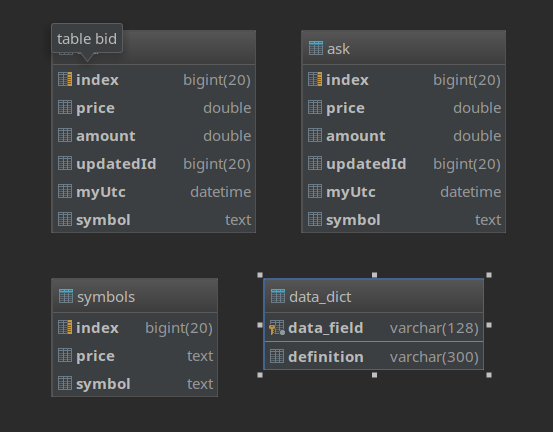
\includegraphics[scale=0.40]{schema.png}
  \caption{Schema}
  \label{fig:schema}
\end{figure}

The tables can be dropped using the ``rollback\_db.sql`` file. This file provides a logical inverse to the create operation. Additionally, I built functionality that can create table on fly using Pandas and SQL Alchemy however the default behaviours are not very good as it fails to create foreign keys and so on.

\subsection*{Tables}
\paragraph*{symbolRef.} This is just a reference table for symbols. The symbols are strings, however it is more efficient to use integers for foreign keys and it is better to store integers than strings.
\paragraph*{bid and ask.} These to table are identical from data types point of view however the just store the bid and ask prices as well as my UTC time stamp and the server `updatedId` flag. This is a large integer that gets changed each time there is a trade.
\paragraph*{limits.}. Basically, the exchange give users request or order limits in time intervals. We can make 1200 data request in a minute or 10 orders in a second and 100 000 orders in a day. If we are creating a real trading application we would have to consider these closely.
\paragraph*{data\_dict.} This is manually created table and holds descriptions for the data fields in the database.

\section*{Bid and Ask}
Bid and ask prices are split into two tables. The tables are identical. The tables from Figure \ref{fig:ask} and Figure \ref{fig:bid} carry the data for the symbol and specific Exchange ID as given by \textit{updateId} column. My time stamps are in the \textit{myUtc} column representing the time on my computer.

\begin{figure}[h!]
	\centering
  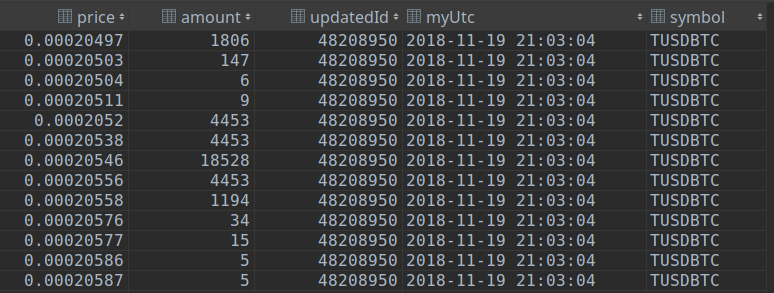
\includegraphics[scale=0.3]{ask.png}
  \caption{Ask Price}
  \label{fig:ask}
\end{figure}

\begin{figure}[h!]
	\centering
  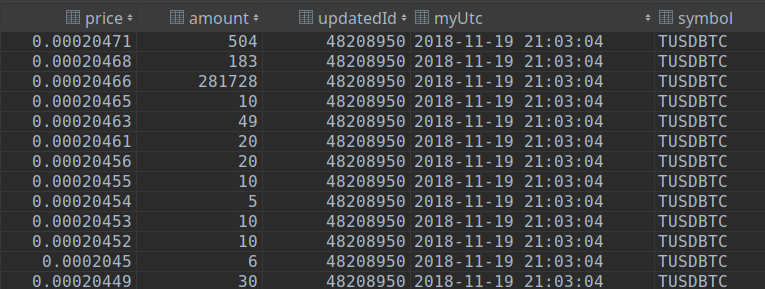
\includegraphics[scale=0.3]{bid.png}
  \caption{Bid Price}
  \label{fig:bid}
\end{figure}

\section*{Exchange API}
It is important to handle the communication to the Exchange well. The class \textit{DataEndPoint} hold all methods that can collect the data from the exchange as opposed to submit trades. I leave it to the reader to read over the comments for these methods to see what can be easily pulled out from the exchange.

\section*{Data Analysis - First Look}
I collected 1 hour of trading data on per second basis. Figure \ref{fig:plt1} shows cumulative bid and ask prices with quantity. The way how I think about this is it is supply and demand curves. We see that there is a lot of volatility over 1 minute interval. This is good as it means that we will be able to create strategies.
\begin{figure}[h!]
	\centering
  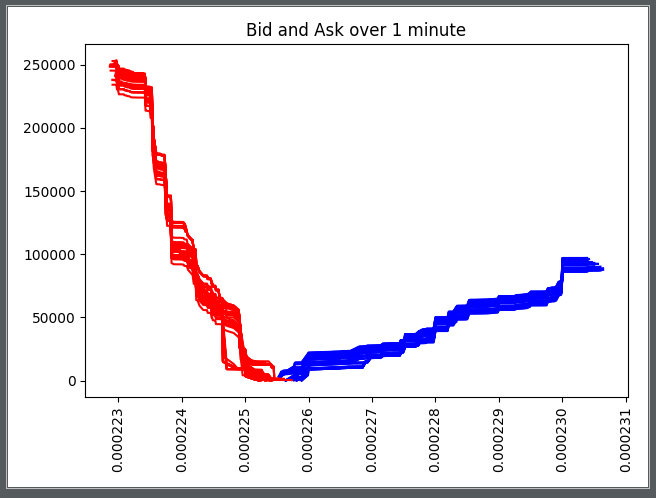
\includegraphics[scale=0.5]{plot1.png}
  \caption{All bid and ask prices and quantities in 1 minute}
  \label{fig:plt1}
\end{figure}

The problem in the Figure \ref{fig:plt1} is that we do not see much details. So, I plotted the same time interval but with close look at what was happing around the spread in Figure \ref{fig:plt2}. Again we see the volatility in the price within one minute.

\begin{figure}[h!]
	\centering
  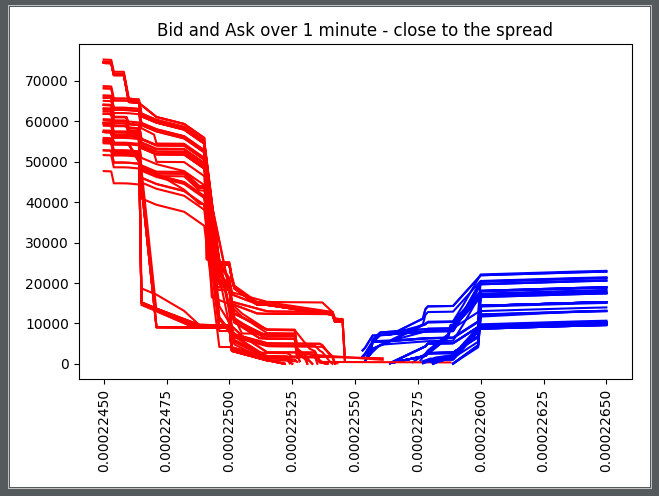
\includegraphics[scale=0.5]{plot2.png}
  \caption{Detailed Price and quantity moments around the spread in 1 minute}
  \label{fig:plt2}
\end{figure}

We also have have look the maximum bid and minimum ask prices and plot them over the 1 hour interval. This is plotted in Figure \ref{fig:plt3}. This shows that we do have trends and turning points happing over time again. We should use the trading strategies that we learning for this and we can starting simulating the trade at bid and ask prices.

\begin{figure}[h!]
	\centering
  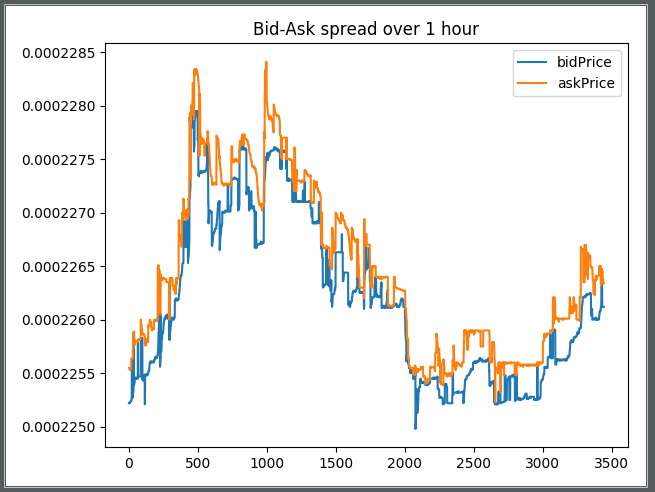
\includegraphics[scale=0.5]{plot3.png}
  \caption{Max bid and min ask over 1 hour}
  \label{fig:plt3}
\end{figure}

Finally, we check the spread for the two currencies as in Figure \ref{fig:plt4}. We immediately see that that we could create mean reversion strategy for the spread. It may not be viable on profit versus fee basis however we could tests this.

\begin{figure}[h!]
	\centering
  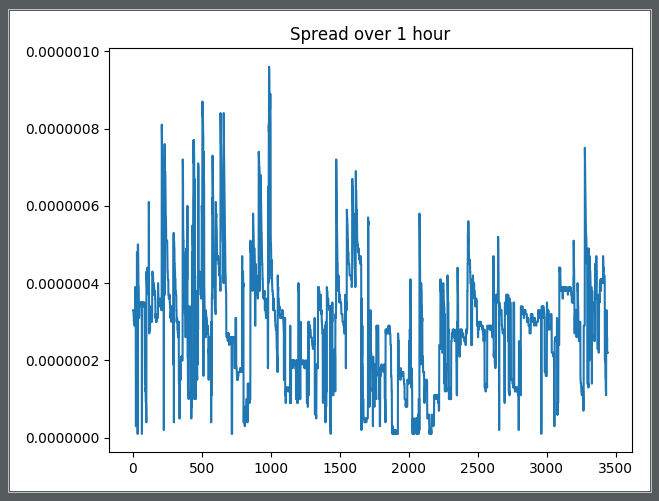
\includegraphics[scale=0.5]{plot4.png}
  \caption{Max bid and min ask spread over 1 hour}
  \label{fig:plt4}
\end{figure}

\section*{Model}
I tried to create my own supply and demand  model as implied in the market order book. That is the model would suggest to us when there is a large deviation from market equilibrium. I thought about market middle price, $P_{mid}$, as
\[
	P_{mid} = \frac{Bid_{max} + Ask_{min}}{2}
\]
where $Bid_{max}$ is the maximum bid price for a given tick and $Ask_{min}$ is the minimum ask price for the same tick.

The idea of my supply and demand estimator should oscillate around this middle price based on the current supply and demand. I attach a probability weights to each supply and demand amounts (see Figure \ref{fig:plt1} and \ref{fig:plt2} to get some feel for what the cumulative amounts look like). I assumed that the probability of arrivals of new orders follows log-normal probability where the orders arriving close to the maximum bid and minimum ask prices are most likely and as we go away from the this bid and ask spread, the arrival of new orders is less likely so they carry small probability weight.

More specifically, I used maximum likelihood estimator for mean, $\mu$, and standard deviation, $\sigma$, for the log normal distribution.
\[
	\hat{\mu} = \frac{1}{n} \sum_{i=1}^{n} \ln{(x_i)} \text{  ,} \quad \hat{\sigma} = \sqrt{\frac{1}{n-1} \sum_{i=1}^{n} [\ln{(x_i)} - \hat{\mu}]^2 }
\]
where $x_i$ is the bid or ask price for the given state of the order book. I assumed that the bid prices and ask prices are independent and they both come from a log normal distribution that is estimated using the current bid and ask prices separately.

We then use the relationship between log-normal and normal distribution to find the probabilities for each prices quoted in the order book. We can use the below to find the probability,  $P_x$, of a given price level to occur.
\[
	P_x = F(x; \mu, \sigma) = \Phi \left( \frac{ln{(x)} - \mu}{\sigma} \right)
\]
with $\Phi$ being the standard normal cumulative density function, see \cite{bury} for details. Considering the shape for the probability density, we know what it is suitable for the ask prices, however I simply reverse the order of the probability mass programmatically for the bid prices to achieve the notion that the prices close to bid are more likely to occur. I then find the expected bid and ask amounts, $a$, as
\[
	\mathbb{E}[a] = \sum_{i=1}^{n} P_{x_i} a_i
\]
We then have a single number that is representing supply and demand that is probability weighted towards the current bid and asks. Further, I define total supply, $S_T$, and total demand, $D_T$ as the sum of the amounts for bid and ask.

As suggested, I tried to define and oscillator around the middle price. I used the price adjustment, $PA$, as

\[
	PA_{ask} = \frac{\frac{S_T + P_T}{2} - (\mathbb{E}[a]_{Demand} - \mathbb{E}[a]_{Supply})}{S_T + P_T} \times \left(\frac{Ask_{min}}{Bid_{max}} - 1 \right)
\]
and
\[
	PA_{bid} = \frac{\frac{S_T + P_T}{2} - (\mathbb{E}[a]_{Supply} -\mathbb{E}[a]_{Demand} )}{S_T + P_T} \times \left(\frac{Ask_{min}}{Bid_{max}} - 1 \right)
\]
\\
When $\mathbb{E}[a]_{Demand}$ is greater than $\mathbb{E}[a]_{Supply}$ I compute 
\[
  \text{adjusted price} = P_{mid} / (1 + PA_{bid})
\]
and otherwise,
\[
  \text{adjusted price} = P_{mid} * (1 + PA_{ask})
\]
The results of the computation are presented in Figure \ref{fig:strat1}.
\begin{figure}[h!]
	\centering
  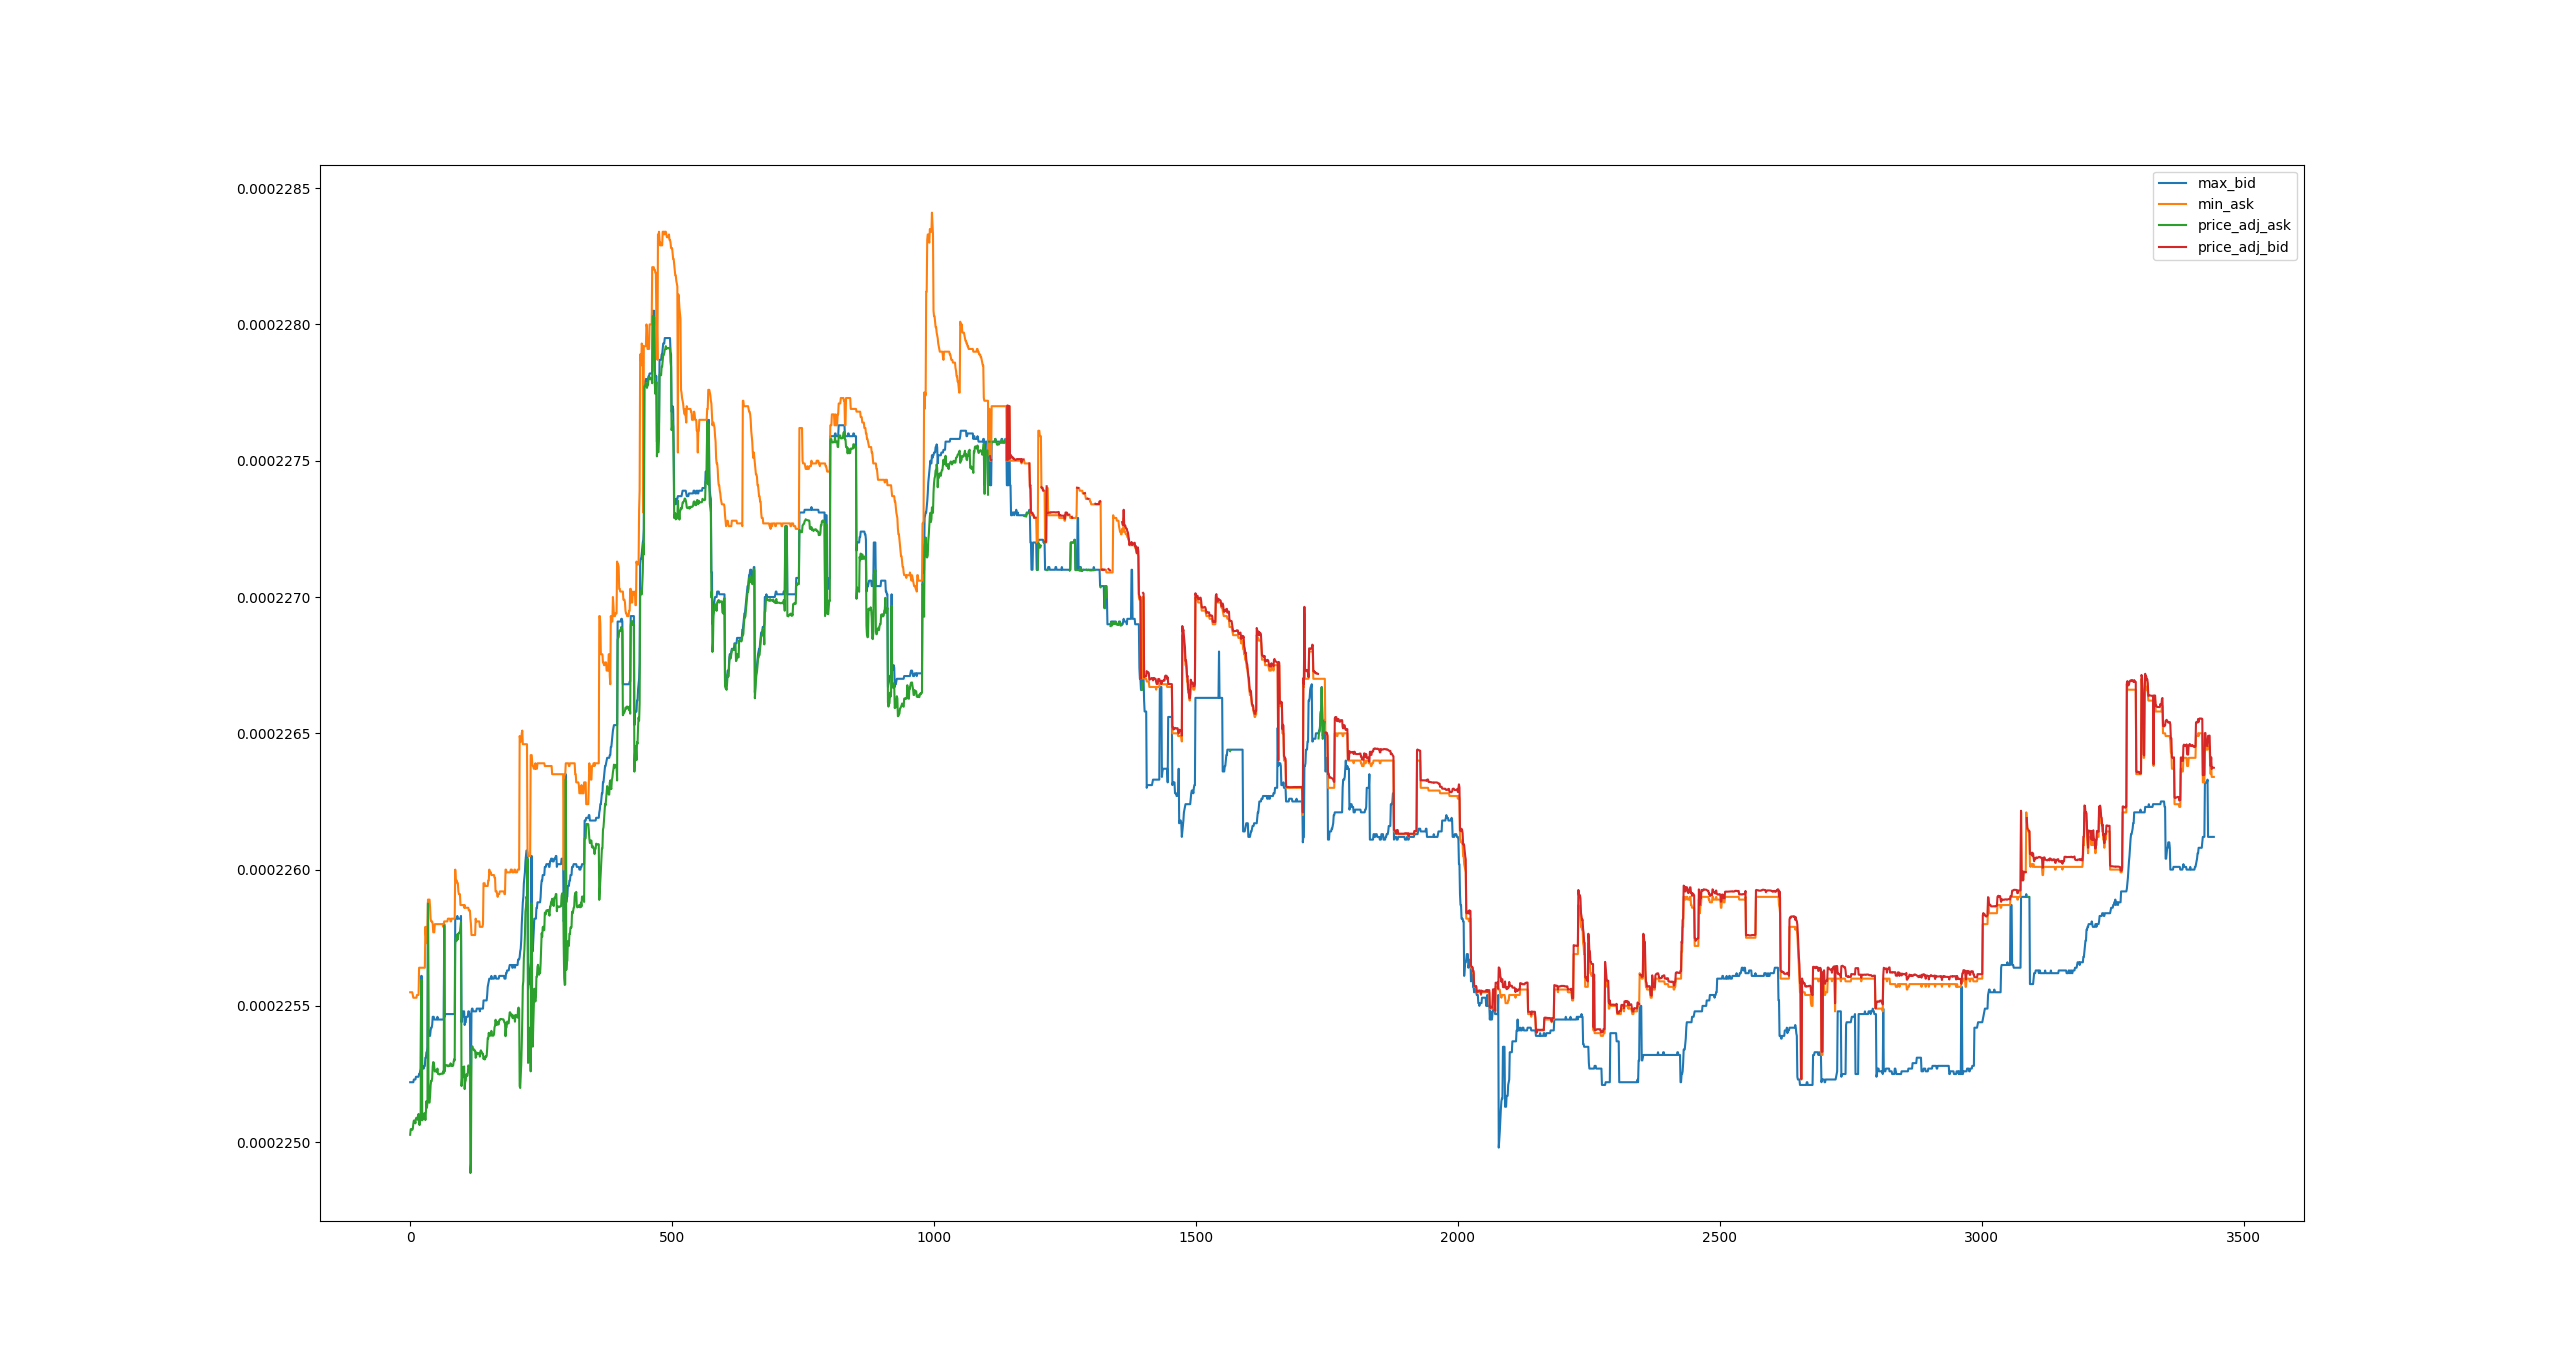
\includegraphics[width=\textwidth]{strategy1.png}
  \caption{Supply and demand indicator}
  \label{fig:strat1}
\end{figure}
We see that in each case my adjusted price is above or below the actual quoted bid or ask. This then suggests that we do not really have an oscillator, we rather indicate where there is a demand stronger and supply. My methods needs further work, however I decided to use the above calculation to design a simple trend following strategy as given in the next section.

\section*{Strategy}
As shown in the Figure \ref{fig:strat1} shows that we could use my model to simple follow the strong demand as an up-trend and strong supply as a down-trend. Figure \ref{fig:strat2} shows frequent switches between the strong supply and strong demand. Perhaps it indicates a small turning point in the market. Then, we do not wish to follow any trend.
Figure \ref{fig:strat4} then show how we can combine the regime switches to a strategy. I used one last minute as an indication as to whether we should take a long a short position.

Figure \ref{fig:strat5} then show the final position. We take a long position, when the market in clearly in the up-trend or wise-versa. We take no position when supply are demand are balanced. The logic for that is

\begin{itemize}
\item Go long when demand is winning over last minute, that at least in last 60 observations, demand was the driver for price at least 55.
\item Go short when in the last 60 observations, at least 57 observations were won by supply.
\item We take no position otherwise.
\end{itemize}
The cumulative returns for this strategy are plotted in Figure \ref{fig:strat6}. The loop for this strategy is shown below.
\pagebreakprint
\begin{verbatim}
    df['position'] = 0
    for n in range(len(df)):
        if n > 60:
            view = df.loc[n-60: n, 'long_signal'].sum()
            if view > 55:
                df.loc[n, 'position'] = 1
            elif view < 3:
                df.loc[n, 'position'] = -1
            else:
                df.loc[n, 'position'] = 0
    # close the trade at the end of the time period
    df.loc[len(df)-1, 'position'] = 0
\end{verbatim}
\FloatBarrier
\begin{figure}[h!]
	\centering
  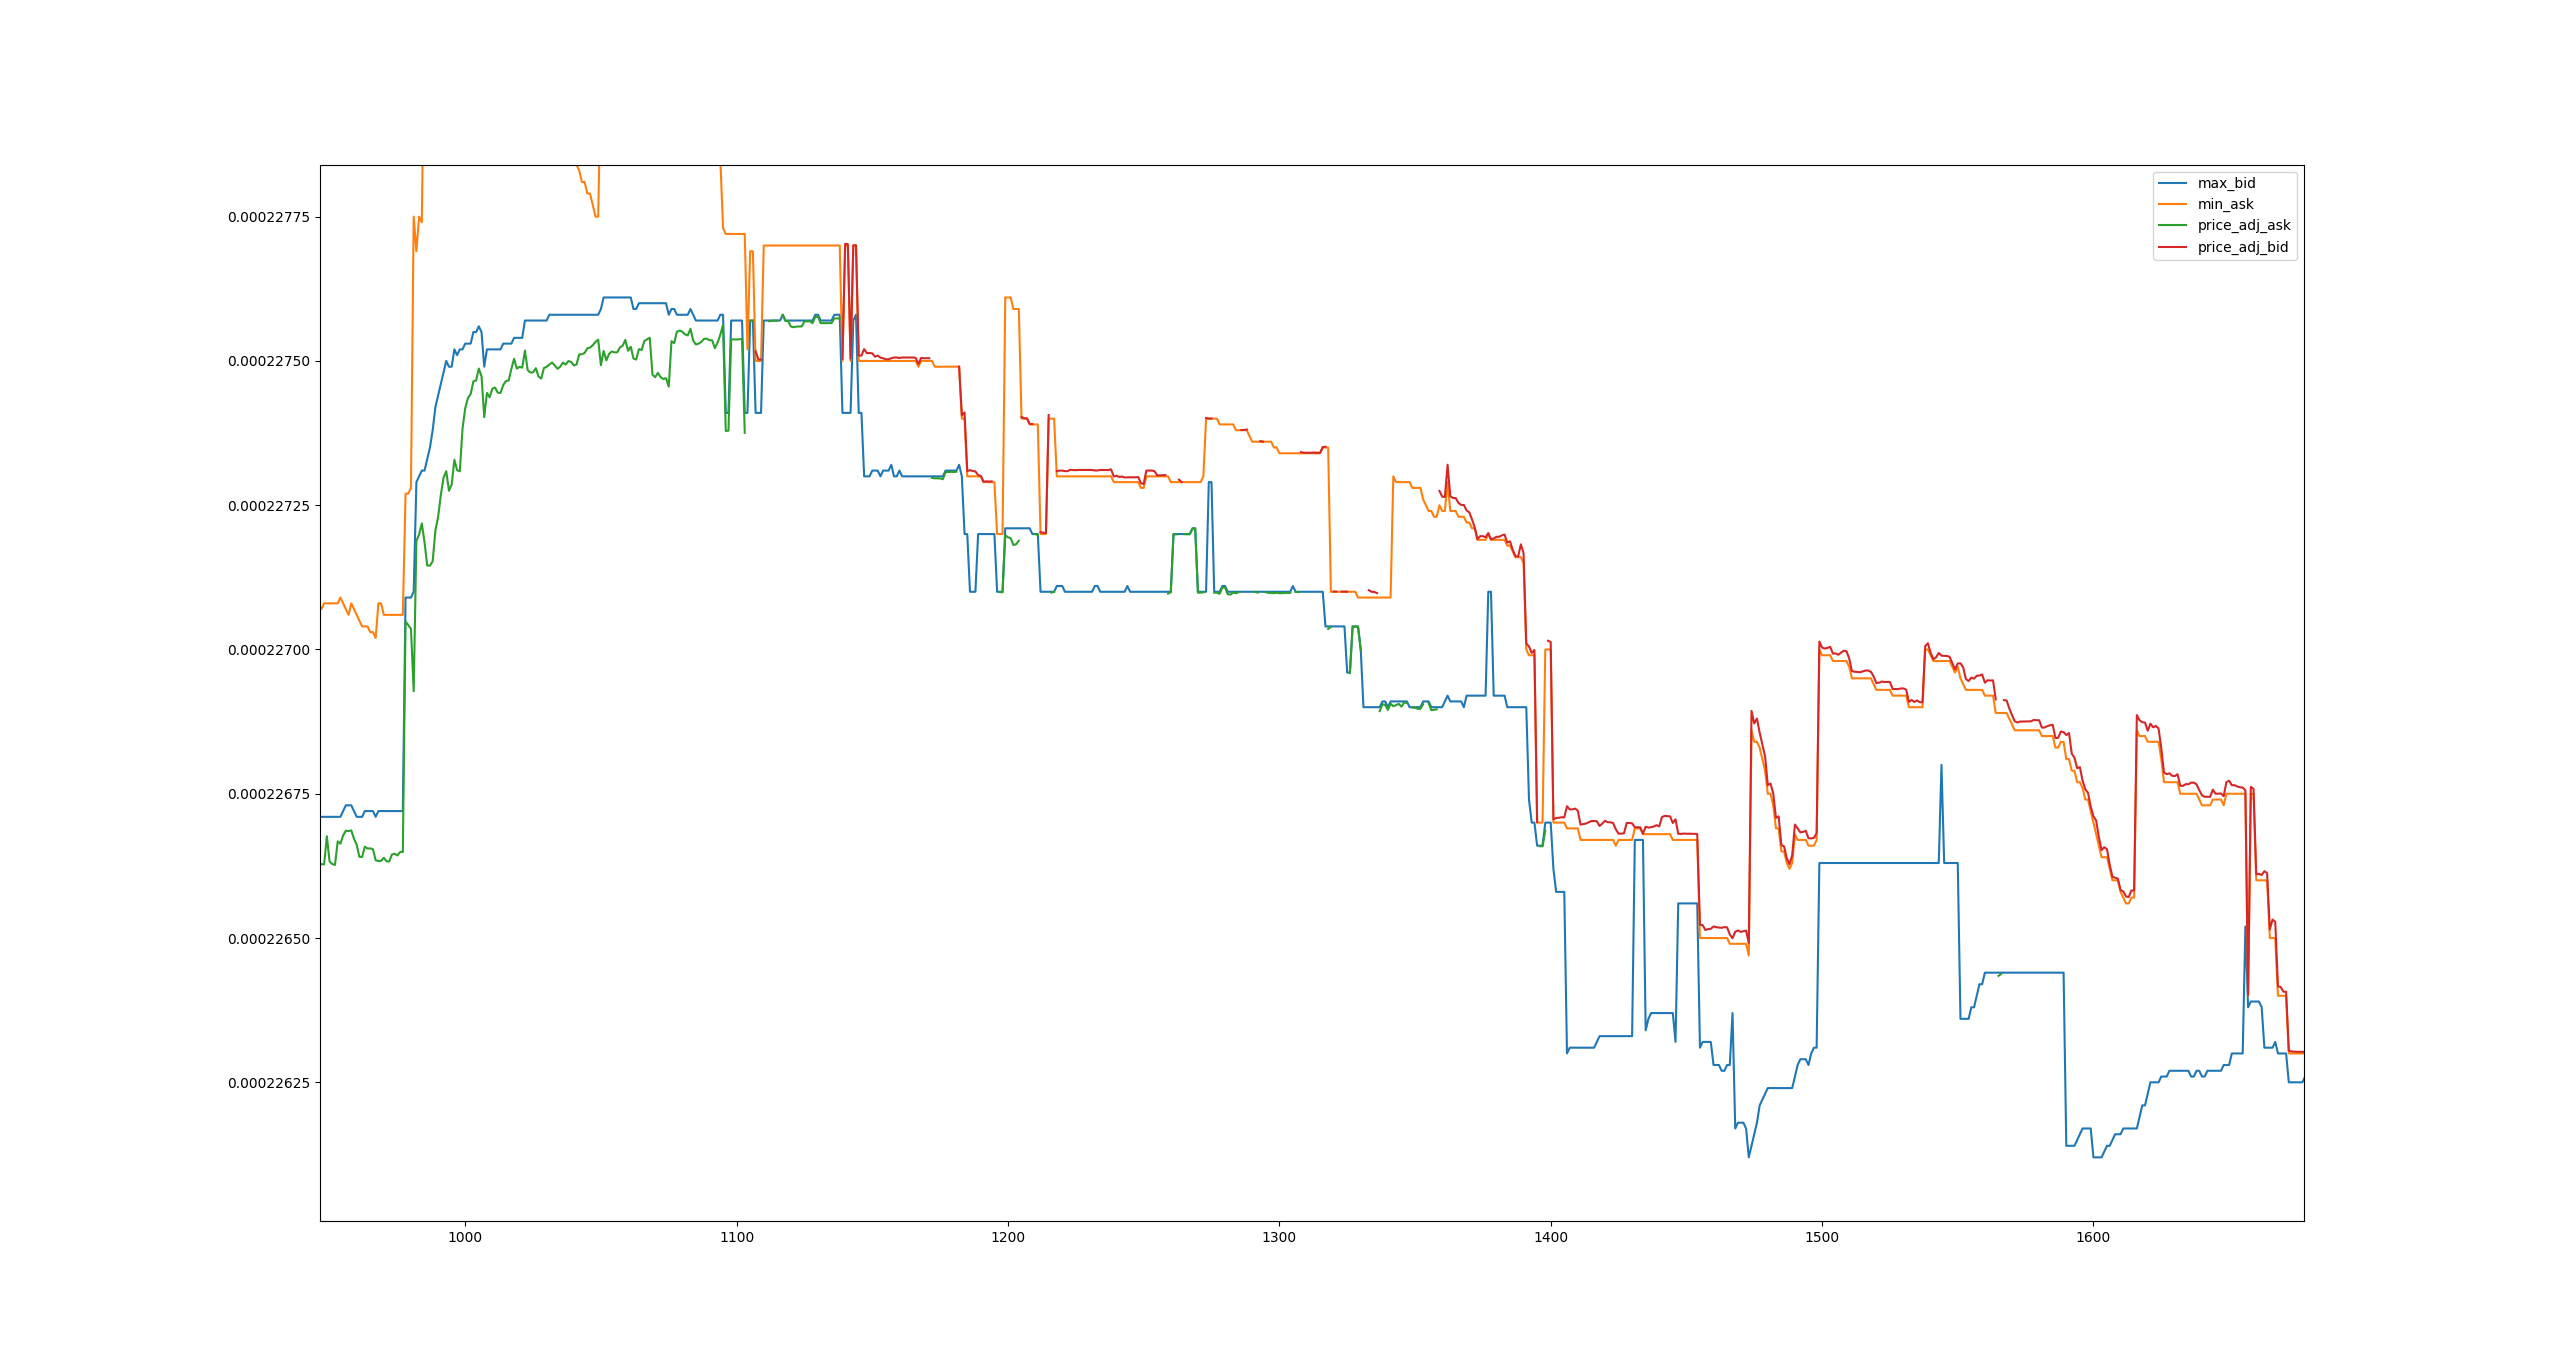
\includegraphics[width=\textwidth]{strategy2.png}
  \caption{Possible turning point}
  \label{fig:strat2}
\end{figure}
Figures \ref{fig:strat3} and \ref{fig:strat4} show the mirrored regime switches. We see that they are identical so we can use just one of them.
\begin{figure}[h!]
	\centering
  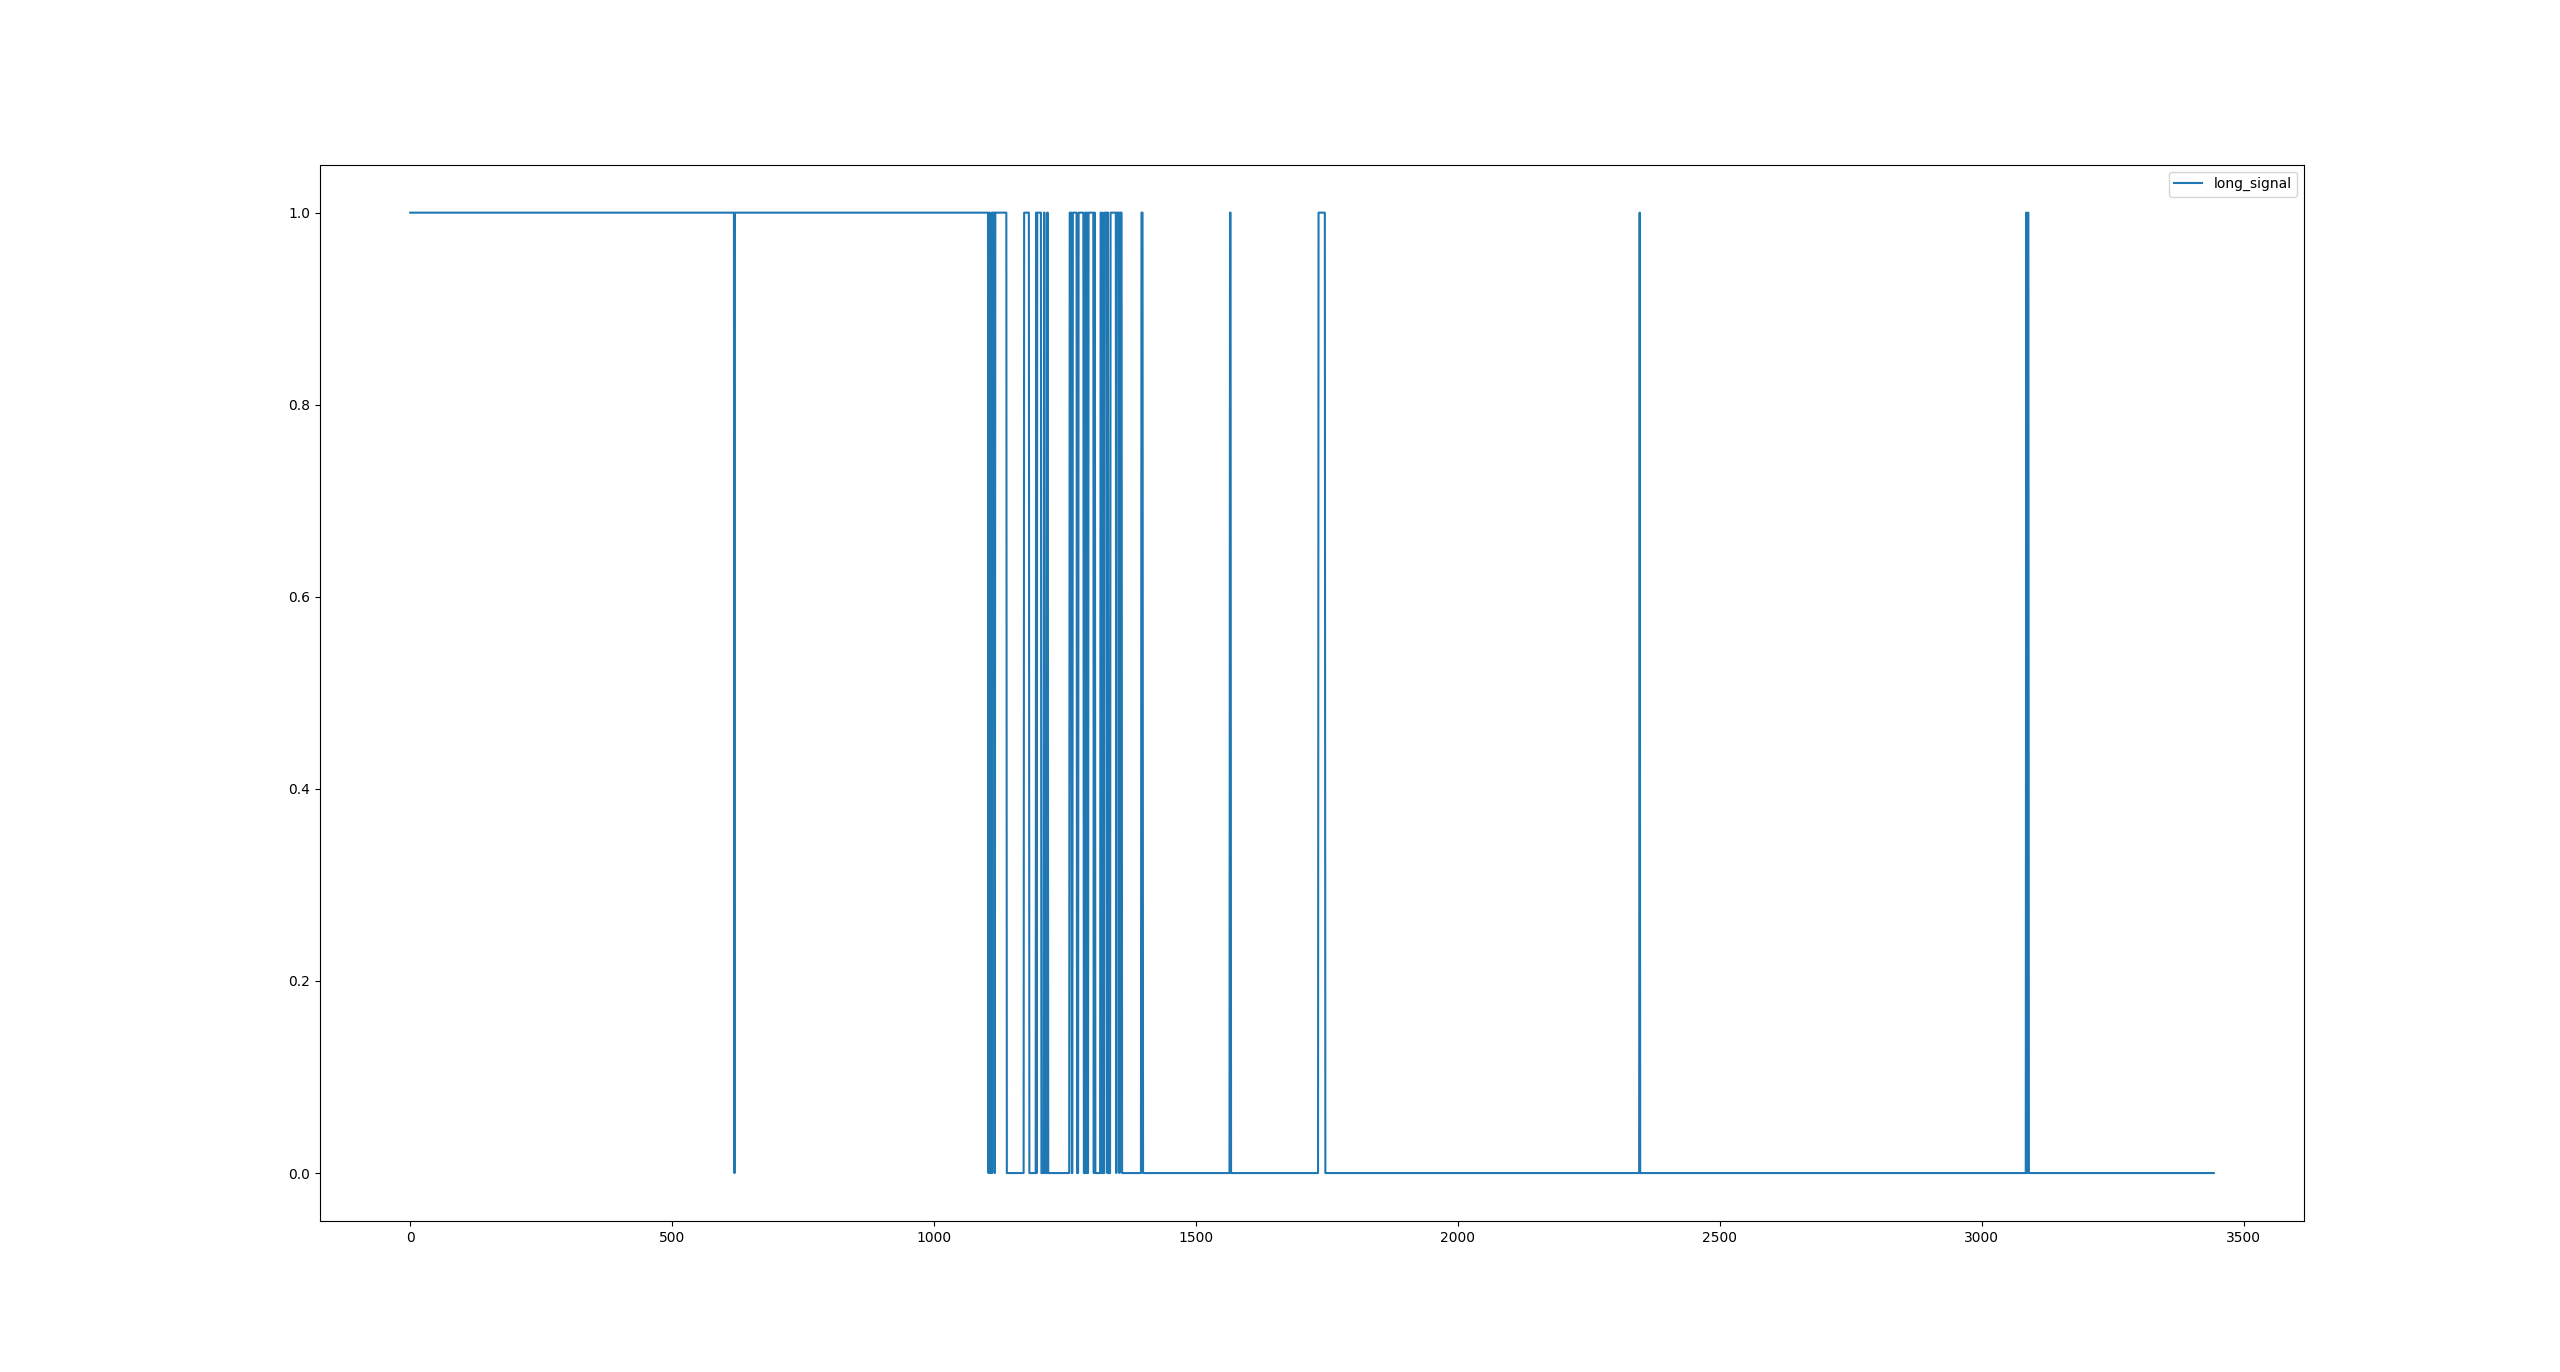
\includegraphics[width=\textwidth]{strategy3.png}
  \caption{Short position indicator}
  \label{fig:strat3}
\end{figure}
\begin{figure}[h!]
	\centering
  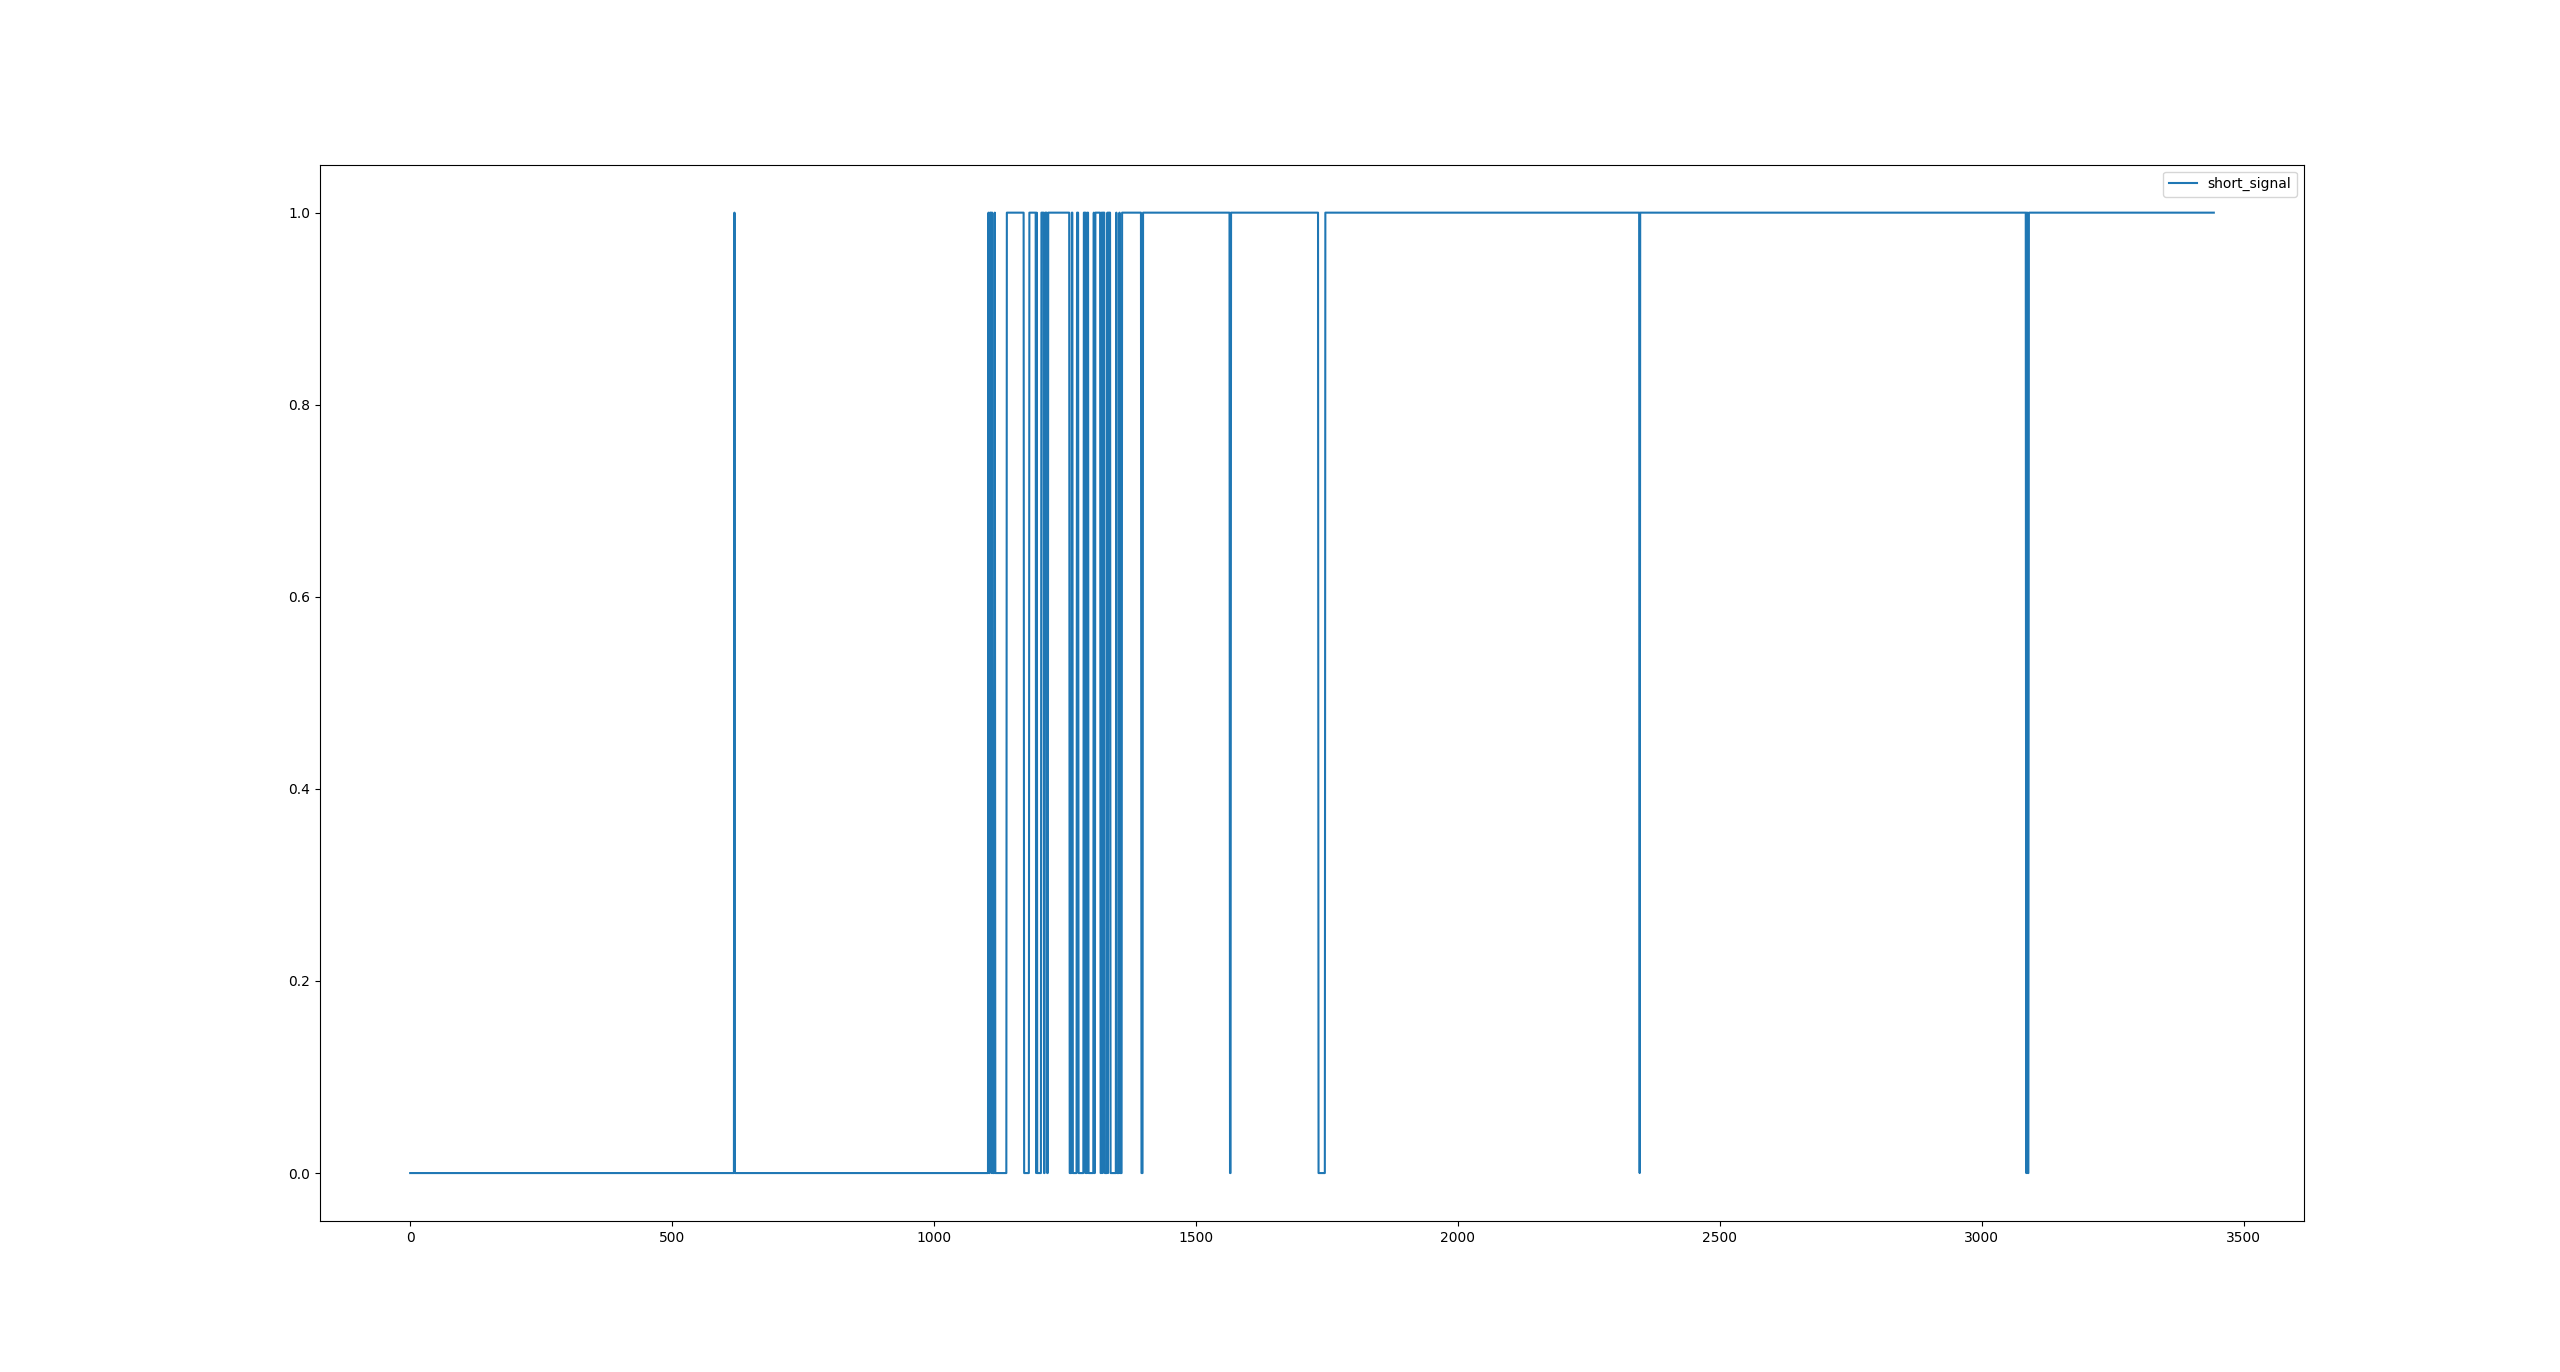
\includegraphics[width=\textwidth]{strategy4.png}
  \caption{Long Position indicator}
  \label{fig:strat4}
\end{figure}
\begin{figure}[h!]
	\centering
  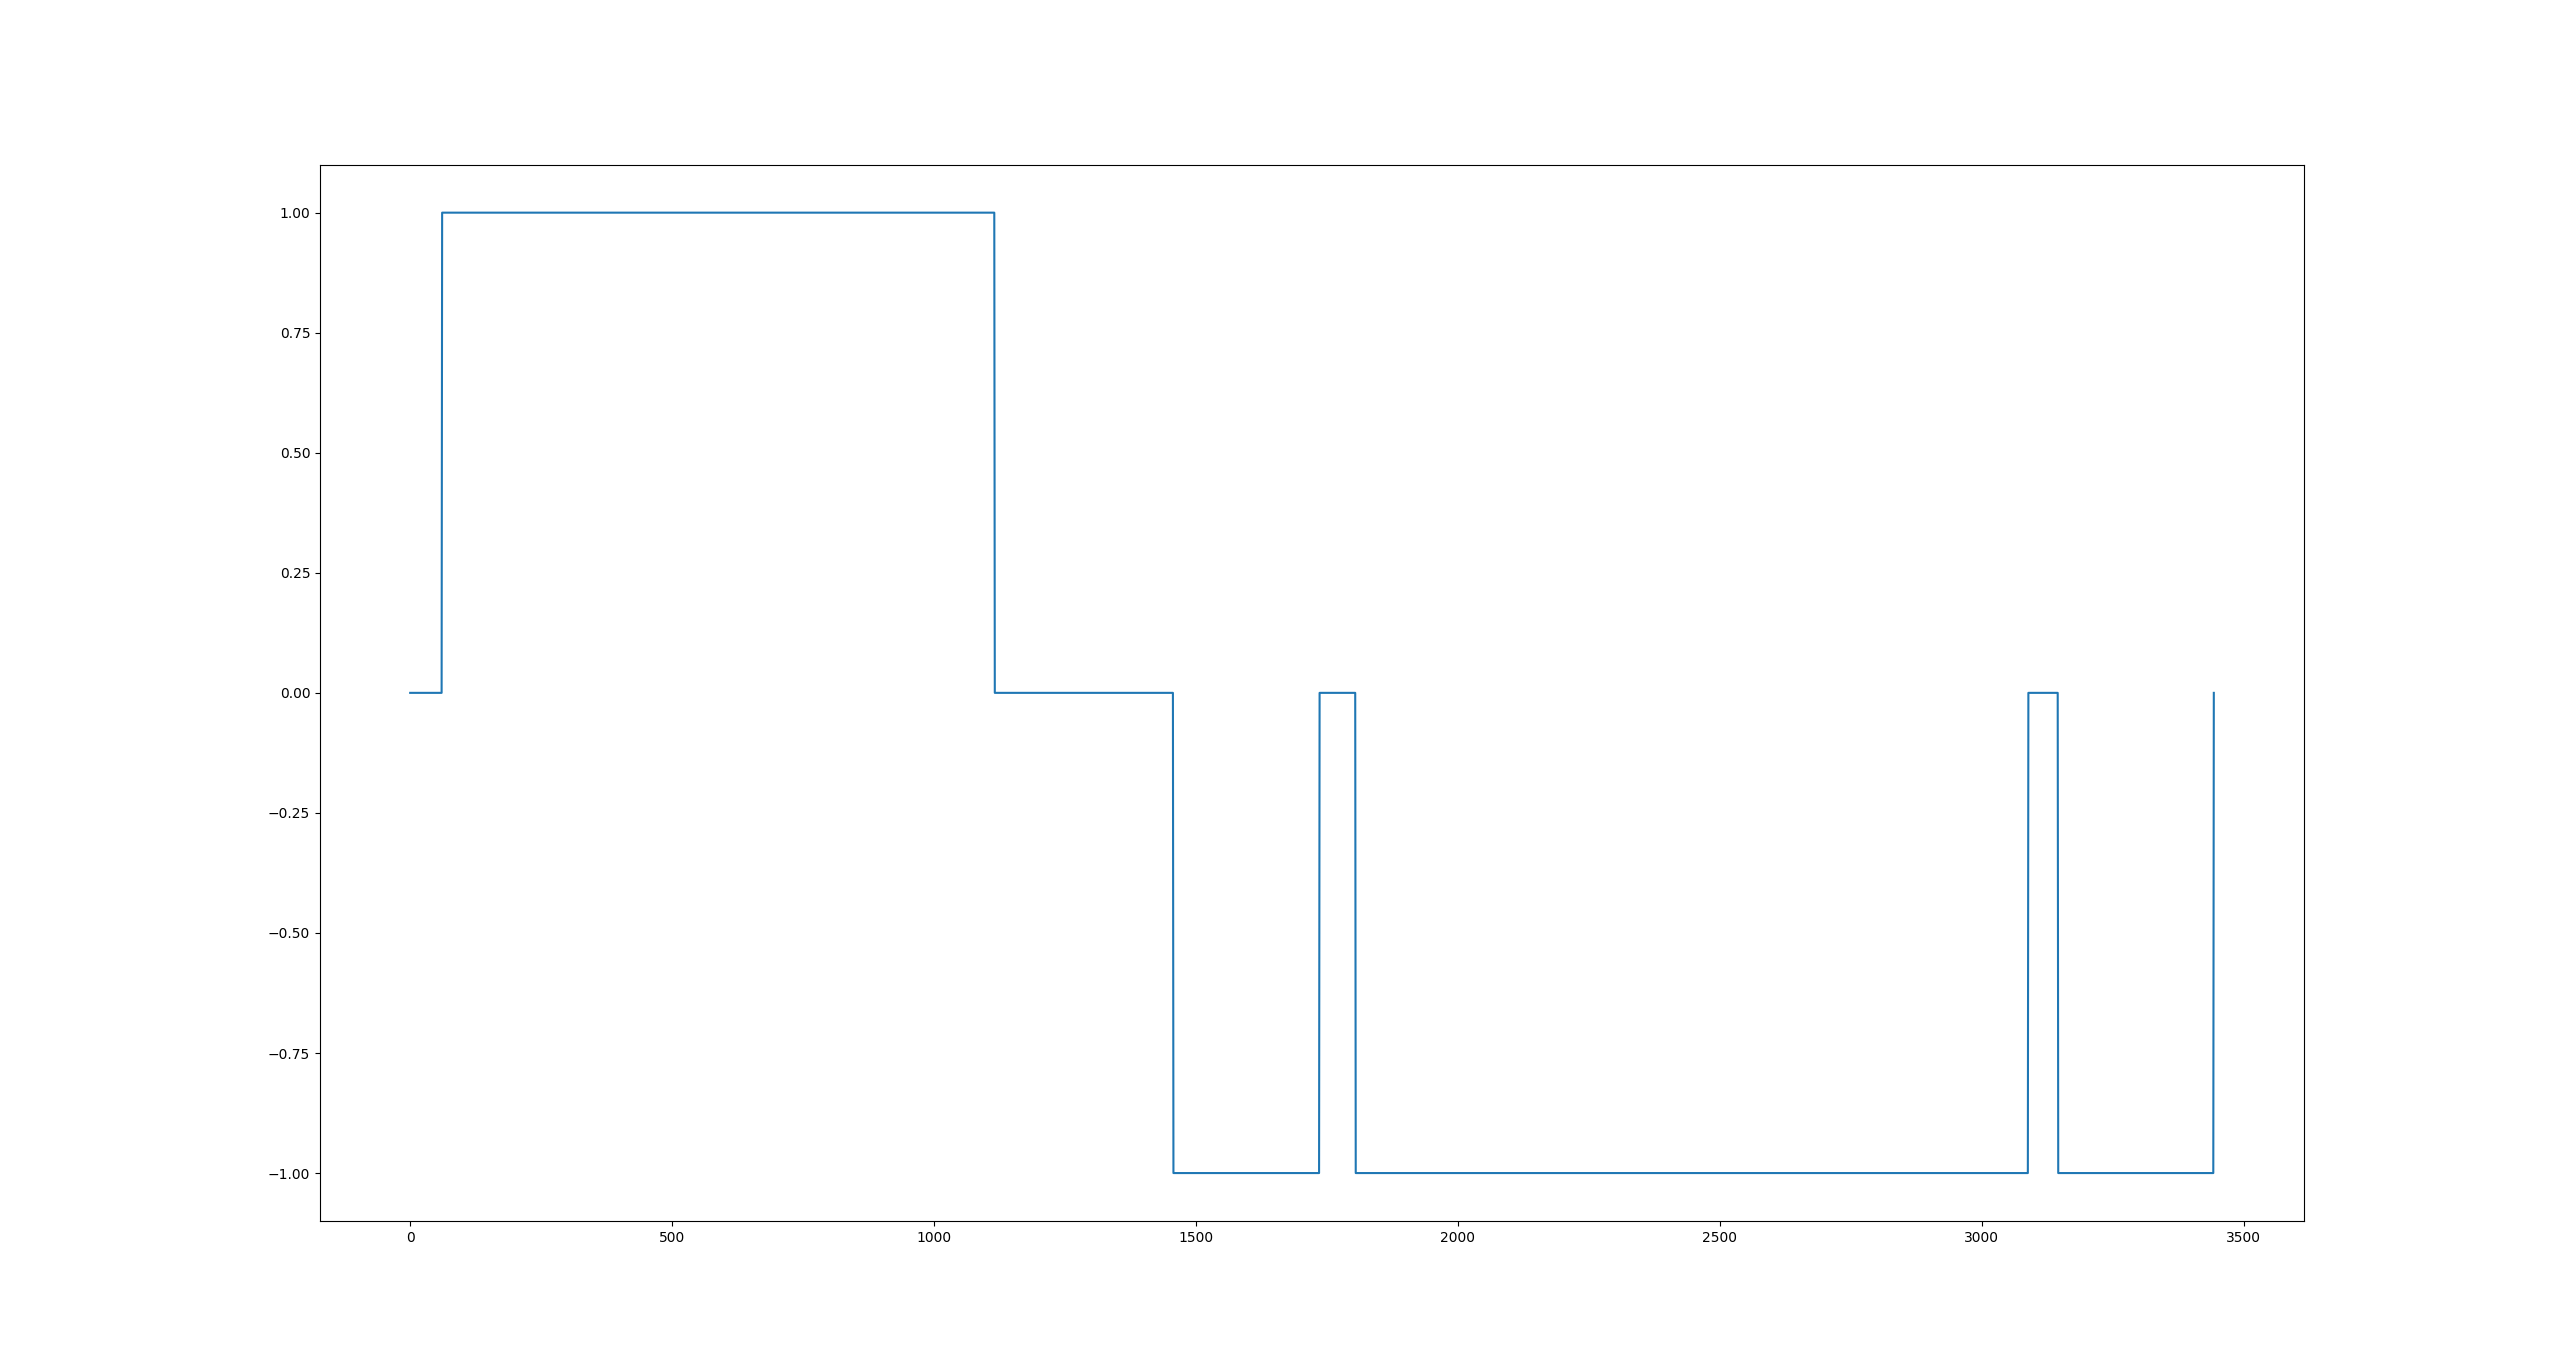
\includegraphics[width=\textwidth]{strategy5.png}
  \caption{Position - Strategy}
  \label{fig:strat5}
\end{figure}
\begin{figure}[h!]
	\centering
  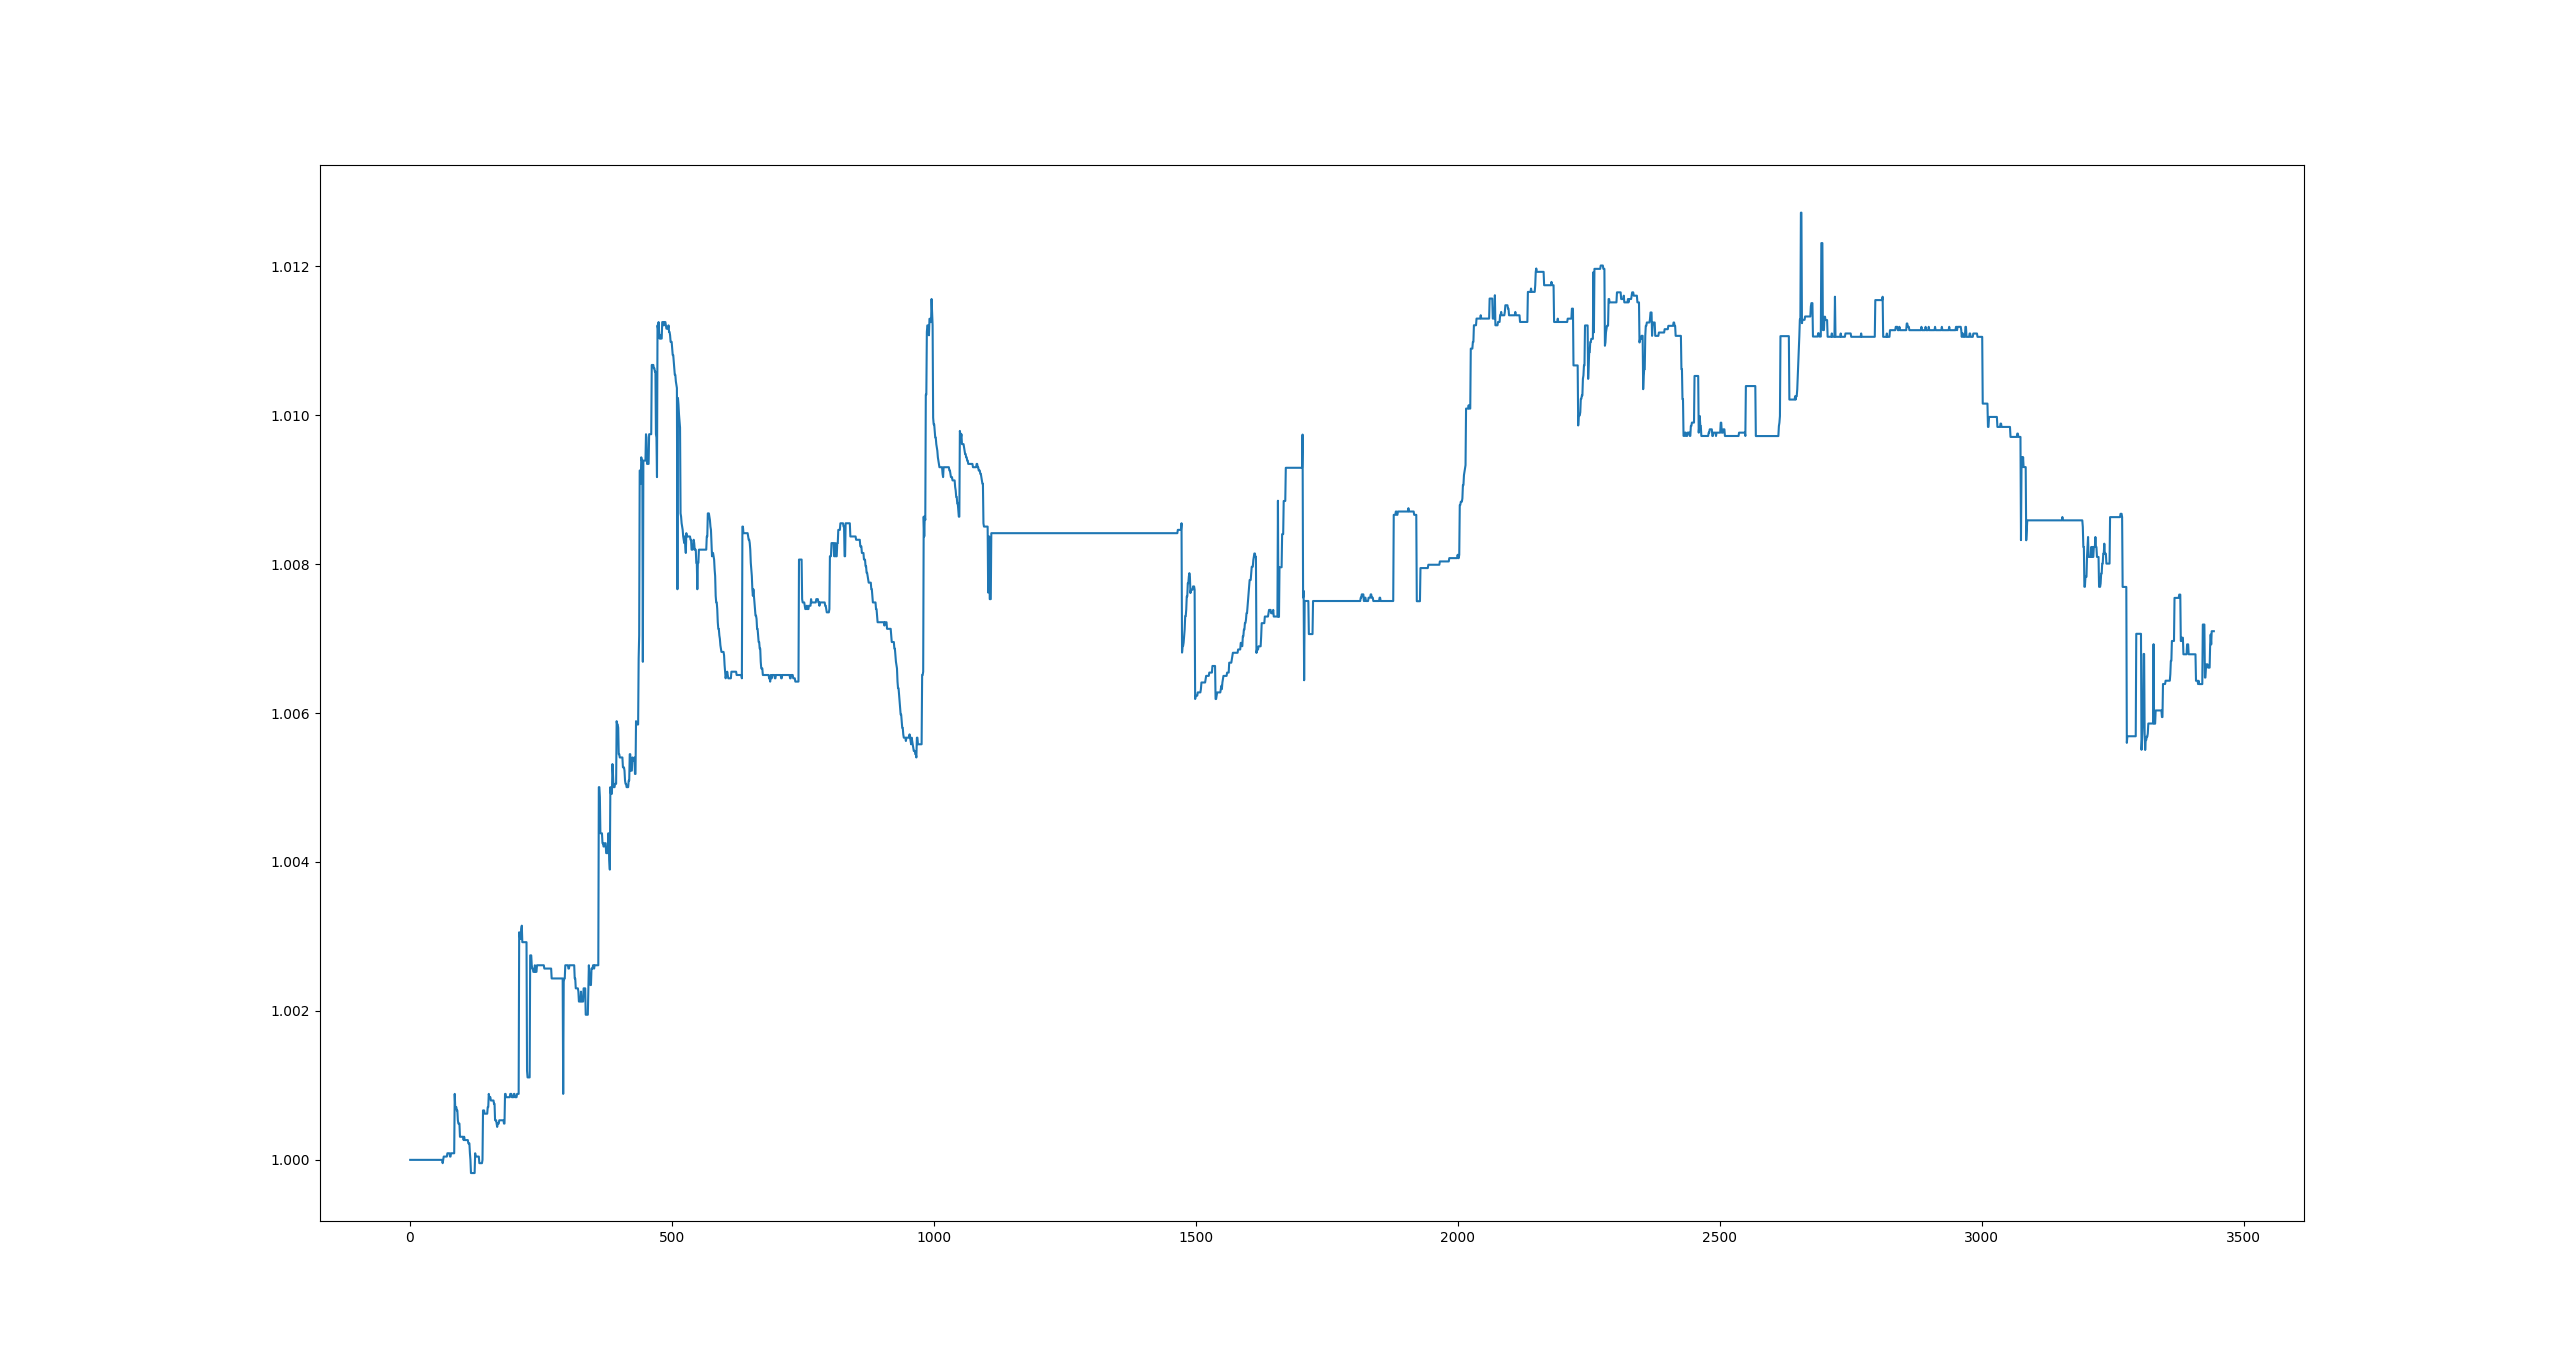
\includegraphics[width=\textwidth]{strategy6.png}
  \caption{Position - Valuation}
  \label{fig:strat6}
\end{figure}

\FloatBarrier
\section*{Strategy Summary}
The KPIs are presented below. We have do a few trades within an hour of trading. KPIs are based on the middle price so it is just an approximation to the performance.

\begin{figure}[h!]
	\centering
  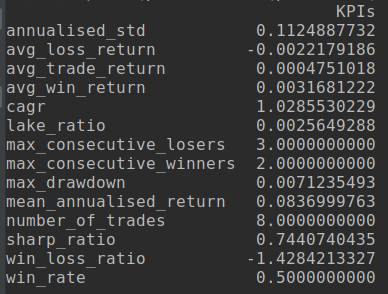
\includegraphics[scale=0.7]{sample_kpis.png}
  \caption{KPI - sample}
  \label{fig:kpi1}
\end{figure}
\FloatBarrier


\pagebreak
\begin{thebibliography}{9}
%  \cite{Template}\label{sec:Chain}

%\bibitem{Template}
%Authors
%\textit{Title}.
%publisher, city, year
%
%\bibitem{knuthwebsite} 
%Knuth: Computers and Typesetting,
%\\\texttt{http://www-cs-faculty.stanford.edu/\~{}uno/abcde.html}

\bibitem{bbc}
BBC 
\textit{Slowing down the predatory high speed traders}.
BBC, UK, 2017

\bibitem{bodek}
Bodek, Haim
\textit{The Problem of HFT}.
CreateSpace Independent Publishing Platform, US, 2013

\bibitem{bury}
Bury, Karl
\textit{Statistical Distributions in Engineering}.
Cambridge University Press, UK, 1999

\bibitem{cbs}
CBS News
\textit{AXA Rosenberg Paying \$242M To Settle Case On Code}.
CBS News, US, 2011

\bibitem{durbin}
Durbin, Michael
\textit{All about high-frequency trading}.
McGraw-Hill, New York, NY, 2010

\bibitem{harris}
Harris, Larry
\textit{Trading and Exchanges: Market Microstructure for Practitioners}.
Oxford University Press, Oxford, 2003

\bibitem{iex}
IEX
\texttt{https://iextrading.com/developer/docs/https://iextrading.com/developer/docs/}, last visited \today

\bibitem{itg}
Investment Technology Group
\textit{Global Execution Strategies}.
Dublin, Ireland, 2013

\bibitem{johnson}
Johnson, Barry
\textit{Algorithmic trading \& DMA: An introduction to direct access trading strategies}.
4Myeloma Press, London, UK, 2010

\bibitem{kirli1}
Kirilenko, Andrei
\textit{HFT Latency Regulation}.
London, UK, 2016

\bibitem{kirli2}
Kirilenko, Andrei; Lamacie, Guilherme
\textit{Latency and Asset Prices}.
London, UK, 2015

\bibitem{kumar}
Kumar, Ganesh
\textit{High Frequency Trading systems and Latency measurements}.
London, UK

\bibitem{lockwood}
Lockwood, John W., Madhu Monga
\textit{Implementing Ultra-Low-Latency Datacenter Services with Programmable Logic}.
IEEE Computer Society, US, 2016

\bibitem{lse}
London Stock Exchange
\textit{A guide to London Stock Exchange 
trading services for equity securities}.
London, UK, 2015

\bibitem{nyse}
NYSE
\texttt{https://www.nyse.com/market-data/real-time}, last visited \today

\bibitem{nytimes}
NY Times
\textit{Knight Capital Suffers Power Failure}.
NY Times, US, 2012

\bibitem{ohara}
O'Hara, Maureen 
\textit{High frequency market microstructure}.
Juournal of Financial Economics, NY, 2014

\bibitem{patterson}
Patterson, Scott
\textit{Dark Pools: The Rise of the Machine Traders and the Rigging of the U.S. Stock Market}.
Crown Business, London, UK, 2013

\bibitem{bapi}
Python-Binance
\texttt{https://python-binance.readthedocs.io/en/latest/index.html}, last visited \today

\bibitem{reuters}
Reuters
\textit{HFT Debate With Haim Bodek and Manoj Narang}.
Reuters, US, 2014

\bibitem{rsj}
RSJ
\texttt{https://www.rsj.com/en/securities/about-us}, last visited \today

\bibitem{vpro}
VPRO
\textit{Flash Crash 2010 - VPRO documentary}.
VPRO, US, 2012

\end{thebibliography}

\end{document}




















